\documentclass[11pt]{article}
\usepackage{graphicx} % This lets you include figures
\usepackage{hyperref} % This lets you make links to web locations
\usepackage[margin=0.5in]{geometry}
\usepackage[rightcaption]{sidecap}
\usepackage{subcaption}
\usepackage{wrapfig}
\usepackage{float}
\usepackage{imakeidx}
\usepackage{indentfirst}
\makeindex
%---------------------------Do Not Edit Anything Above This Line!!------------------------

% edit the line below, if needed, to change the directory name for your image files.
\graphicspath{ {./diagrams/} }



\begin{document}

%---------------------------Edit Content in the Box to Create the Title Page--------------
\begin{titlepage}
   \begin{center}
       \vspace*{1cm}
	   \Huge
       \textbf{Rampage Technical Document}

       \vspace{0.5cm}
       \Large
       Sprint 4 \\
       12/1/2023 \\
   \end{center}

       \vspace{1.5cm}

\begin{table}[h!]
\centering
\begin{tabular}{|l|l|}
\hline
\textbf{Name} & \textbf{Email Address} \\ \hline
Andrea Florence         & andrea.florence180@topper.wku.edu         \\ \hline
Tameka Ferguson         &tameka.ferguson183@topper.wku.edu          \\ \hline
Shikha Sawant         & shikha.sawant059@topper.wku.edu         \\ \hline
Aaron Beasley         & aaron.beasley908@topper.wku.edu         \\ \hline
\end{tabular}
\end{table}

%Latex Table Generator    
%https://www.tablesgenerator.com/     
        
\vspace{4in}

\centering        
CS 360 \\
Fall 2023\\
Dr. Michael Galloway\\
Project Technical Documentation

\end{titlepage}
%---------------------------Edit Content in the Box to Create the Title Page--------------


% No text here.


%---------------------------Do Not Edit Anything In This Box!!------------------------
%Table of contents and list of figures will be autogenerated by this section.
\newpage
\setcounter{page}{1}%
\cleardoublepage
\pagenumbering{gobble}
\tableofcontents
\cleardoublepage
\pagenumbering{arabic}
\clearpage
\newpage
\setcounter{page}{1}%
\cleardoublepage
\pagenumbering{gobble}
\listoffigures
\cleardoublepage
\pagenumbering{arabic}
\newpage
%---------------------------Do Not Edit Anything In This Box!!------------------------




%---------------------------Project Introduction Section------------------------------

% No text here.

\section{Introduction} %\section{} is used to create major section headers

% No text here.

%---------------------------Project Overview------------------------------------------
\subsection{Project Overview} %\subsection{} is used to create minor sections 
% 300 words
% Description of the project, what the project provides, its purpose, problems solved, and target audience.
The main goal of this project is to recreate one level of the game Rampage as close to the original as possible. We created the game with accurate an player sprite and NPC sprites as close to the original as possibe. The player sprite was found through Spriters Resource, the NPCs were drawn in an online pixel art maker by Andrea. We ulitmately decided to use the night edition of the game for the background. The gameplay mechanics are largely button presses, meant to mimic the way the game was actually played on arcade machines. It is as non-reliant on screen touching as possible. The sound effects of the original game were also hard to find, leading us to take creative liberty and use our own created audio for this project. With limited resources on the table, we were prepared to do whatever it took to find the best substitutes to make our remake close to the original as we could. 

Our client and audience, Dr. Galloway also informed us to document anything we completed in our project so that he could be sure that everyone in our group has done our part, as well as ensure that the project could be replicated by anyone given the documentation. All members were expected to use Unity at the client's request. We wre also tasked with creating a Gantt chart to stay organized and document the times that we spent working on our project. This project provides users with a game that challenges hand-eye coordination. Players must be able to think about plans of action in order to collide with the buildings without coming into contact with any NPCs. The game was made in Unity and shared with other members of the team.There is a built-in sign in/sign up system for the player to create an account and land their score on the leaderboard. We also took security measures to ensure that the player does not have the power to cheat the game like actual console games do.


 

%---------------------------End Project Overview---------------------------------------

% No text here.

%---------------------------Project Scope----------------------------------------------
\subsection{Project Scope}
% 350 words
% Description of all deliverables, benefits, outcomes, and work required (all tasks, costs, time, people, resources, dates/deadlines, and final deliverables date).

The scope of this project included the writing of two written reports, the technical and organizational documents, a presentation, and a CATME evaluation. The technical document includes the project overview, scope, requirements, model and design, non-functional details, and testing of software. The organizational document includes the team’s organizational approach, task schedule, team’s known progress in project, and managing possible risks. The presentations focus on giving the client an overview of project, progress on project and future plans. The CATME evaluations let client know how each team member contributes to project, how team members interact with each other, if the team members check on each other’s progress, and overall interactions with the project. 
The benefit for this project is to acquire skills pertaining to software engineering. This entails learning how to analyze requirements, determining the needs for a desired project outcome, user interface, design, construction, testing and maintenance. Along with this, we got to do this with a team who is also learning as the project progresses. As a team, we expected that the outcome for this project would be that we are able to successfully remake a level of Rampage as close to the original game as possible. 

The tasks for the project were to comple the technical and organizational documentations, the presentations, evaluations and the final product. With documents, each team member was given a specific part of the document that they had to make contributions to and complete. The presentations were created based on the technical and organizational documents that we had completed. The evaluations were be done once preparations for the presentation have been made. The development of the final product startes in Sprint 3. The project was completed at the end of Sprint 4.

There were no costs accumulated for the project other than time cost for each team member. We met every week to discuss future plans and evaluate our current work. The time costs were dependent on the arranging of the team members schedules and changed week by week. Our team consisted of Aaron Beasley, Andrea Florence, Shikha Sawant, and Tameka Ferguson. Unity tutorials and resources, YouTube, and class lectures were the necessary resources for this project. 

Sprint 1 documentation was due on September 7th. The first evaluation and presentation were due on September 4th. 
Sprint 2 documentation was due on October 6th. The presentation and CATME evaluations were due on October 4th.
Sprint 3 documentation was due on November 3rd, and the CATME evaluation was due that day as well. The presentation was due on October 30th.
Sprint 4 documentation was due on December 1st, and the CATME evaluation is due that day as well. The presentation was due on November 27th.


%---------------------------End Project Scope---------------------------------------

% No text here.


\subsection{Technical Requirements}


%---------------------------Functional Requirements----------------------------------------------
\subsubsection{Functional Requirements} %\subsubsection{} used to create sections for parent subsections.
% Functional requirements define what a system or software must do, specifying the desired behavior or functionality.

% List as atomic bullet points that can be tested

\begin{table}[h!]
\centering
\begin{tabular}{|l|}
\hline
\textbf{Mandatory Functional Requirements} \\ \hline
1. Player Controls                               \\ \hline
a. Move left/right and Jump                                \\ \hline
b. Accessing a menu
2. Player Lives                              \\ \hline
a. Player has 3 lives in gameplay.        \\ \hline
3. Player Accounts                                                      \\ \hline
a. How will the players' data be saved? Logging In?             \\ \hline
b. Multiple accounts?                                       \\ \hline
4. NPCS/Vehicles                            \\ \hline
a. Dying from player                             \\ \hline
b. Inflicting Damage                                \\ \hline		 \\ \hline
5. Building 					\\ \hline
a. Disappear upon collision	               \\ \hline
b. Kill NPCs	               \\ \hline
                                           \\ \hline
                                           \\ \hline
\textbf{Extended Functional Requirements}  \\ \hline
1. Injury
a. Programming inflictions         \\ \hline
2. Visuals            \\ \hline
a. Aesthetics             \\ \hline
3. Environment                 \\ \hline
a. Environment size          \\ \hline
b. Building size                     \\ \hline
c. What moves/doesn't move             \\ \hline
4. Graphics                 \\ \hline
a. Color scheme                \\ \hline
                                           \\ \hline
                                           \\ \hline
\end{tabular}
\end{table}

% Paragraph (150 words) explaining the need and purpose for the listed Functional Requirements.
The mandatory functional requirements are needed to actually make a game that has all the bare minimum requirements. The requirements we have listed enable our game to have an objective that makes it unique compared to any other game. In order for the players’ character to interact with the game, it needed to be able to move left and right. We had to ask the questions “How will the player move and climb buildings, and destroy them? What controls can we assign to the computer to do these specific functions?” We used AD and the left and right arrow keys for character movement, and the spacebar to allow the character to jump. Another function that was necessary was a way to track player lives. The question we had to ask is “How much damage can they take before dying?” along with this, another functional requirement was the ability to manage accounts. We had to ask “How many accounts can be made for our game? Will this be a single player or multiplayer?” These were the bare minimum functions that are mandatory to successfully make a functioning game. 


%---------------------------End Functional Requirements----------------------------------------------

% No text here.

%---------------------------Non-Functional Requirements----------------------------------------------
\subsubsection{Non-Functional Requirements}
% Non-functional requirements specify the constraints, qualities, or attributes that the system or software must possess, such as performance, security, usability, portability, fault tolerance, or reliability.

% List as atomic bullet points that can be tested
\begin{table}[h!]
\centering
\begin{tabular}{|l|}
\hline
\textbf{Mandatory Non-Functional Requirements} \\ \hline
1. Implementation                               \\ \hline
a. Using Unity                               \\ \hline
b. Windows software                              \\ \hline
2. Security                 \\ \hline
a. Ensure player cannot cheat                 \\ \hline
3. Metrics                         \\ \hline
a. Hardware metrics TBD                         \\ \hline
4. User Interface                          \\ \hline
a. Buttons will be the main controls                            \\ \hline
                                           \\ \hline
                                           \\ \hline
\textbf{Extended Non-Functional Requirements}  \\ \hline
1. Response Time						  \\ \hline
a. Their movement and design 						  \\ \hline
2. Loading Time                         \\ \hline
3. Compatibility and Accessibility                         \\ \hline
4. CPU/Memory Usage                         \\ \hline
5. Network Performance                         \\ \hline
a. Assuming this game would be accessed online                         \\ \hline
6. Storage                         \\ \hline
a. Progress storage                         \\ \hline
b. Chances of lagging?                         \\ \hline
7. Bugs                         \\ \hline
a. Debugging                         \\ \hline
                               			  \\ \hline
                                           \\ \hline
                                           \\ \hline
\end{tabular}
\end{table}

% Paragraph (150 words) explaining the need and purpose for the listed Non-Functional Requirements.
The mandatory non-functional requirements are the basic requirements that we needed to consider outside of the actual game functionality itself. These pertain to the baseline characteristics on how and where the game will be built and stored upon, as well as other things. It also pertains to different performance times such as response times and loading times. The purpose of studying these requirements is to ensure the performance times are reasonable enough for the enjoyment of the player. Different storages were also types of nonfunctional requirements we had to consider given it shouldn’t be too large for our client’s computer or ours. It was developed in the game engine called Unity since that is what the client requested. The non-functional requirements became clearer the longer we worked and developed the game. We took a bit of leeway in character movement, and in the actual design and graphics of our game and characters within it.

%use blank lines to begin a new paragraph



 
%---------------------------End Non-Functional Requirements---------------------------------------

% No text here.

%---------------------------Target Hardware Details----------------------------------------------
\subsection{Target Hardware Details}
% 300 words minimum
% CPU (if a specific architecture is needed), RAM (required while the product is running), Persistent Storage Space, Network connection (Wi-Fi, Ethernet), Network bandwidth (required while the product is running), Output devices (Monitor (how many? What resolution?), speakers, VR headset), Input devices (Keyboard, mouse, touchscreen, VR headset).  Create test cases for each to verify.
Since the first sprint was mainly about familiarizing ourselves with the project and getting a basic understanding of our task at hand, we didn't begin thinking about the technical requirements until further into the second sprint. We based our target hardware on the assumption that this game will be accessed on Unity, so the hardware of the device that would access the game would need to be able to run Unity. Meanwhile all of our team members were using windows to access Unity, so we also based the details on this fact. 

For our development team, the necessary operating system (OS) needed to run our game was Windows 7 and newer, 64-bit versions only. The CPU had to be x64 architecture with SSE2 instruction set support. The Graphics API had to be DX10, DX11, and DX12 – capable GPUs. Additional requirements were that the members had hardware vendor officially supported drivers. For all operating systems, the Unity Editor is supported on workstations or laptop form factors, running without emulation, container or compatibility layer so we were fine from that point.

For players not running the game from the Unity engine, the system requirements are different depending on what software they intend to play the game on. For Android, the version would have to be 4.4(API 19)+, CPU ARMv7 with Neon Support (32-bit) or ARM64, and Graphics API would be OpenGL ES 2.0+, OpenGL ES 3.0+, Vulkan. For iOS, the version would have to be 11+, CPU A7 SoC+, and Graphics API would be Metal.

The necessary RAM needed for most users when using Unity would be 32GB and 64GB+ for those interested in building lighting which takes more than a few hours. Output devices would be speakers for the in-game sound. Input devices would only be the keyboard to determine the movements and actions of the playable character. 


%---------------------------End Target Hardware Details----------------------------------------------

% No text here.

%---------------------------Software Product Deveopment----------------------------------------------
\subsection{Software Product Development}
% 300 words minimum
% List the following used with their purpose for development: IDEs, IDE plugins, Software Languages, Software Frameworks, Version Control, Asset Generation Tools, and tools for colaboration (Google Drive, One Drive, GitHub, etc.).  Describle how each tool is used within your team.
The IDE we decided to use to program our C-sharp scripts was Visual Studio. Since we used Unity, the default script editor is Visual Studio. All of our team members were also already somewhat familiar with Visual Studio, so it worked best for us to continue with something we already had familiarization with. 

Another option was to use an IDE plugin that has Unity support built in. We considered using JetBrains Rider, which is a C-sharp editor. JetBrains Rider makes writing C-sharp a lot smarter. Since, none of our members had experience in C-sharp, JetBrains Rider could have been very helpful in enhancing our skills and acting as a good IDE plugin. 
The software language that we used in the development of our project was C-sharp since this is the language that Unity used to build games with. Our version control will be Git. Not all of our members were familiar with Git or GitHub either so that was a learning experience for most of the team. We used an online pixel art creator to create some of the assets to use in development within our sccenes.

We used Discord to communicate and share documents for each sprint. Discord is a very convenient social platform that made both connecting and conveying information between our team members more efficient. As we moved onward into the project and began using Unity, we decided to use GitHub for version control to ensure that all team members were aware of changes in our game development and were able to build on the newest edition of the game as it was developed. We commited changes to GitHub as we were editing the Unity file so that we all have the latest version of our software. 



%---------------------------End Software Product Deveopment-----------------------------------------

% No text here.

%---------------------------End Project Introduction Section----------------------------------------


% No text here.





%---------------------------Modeling and Design Section------------------------------
\section{Modeling and Design}
% No text here.


%---------------------------System Boundaries------------------------------
\subsection{System Boundaries}

\subsubsection{Physical}
%150 words minimum
% Describe the Physical System Boundaries.
The hardware components and resources that were used for the software system were the operating system, the CPU, the graphics API and disk space. For android the OS version needs to be 4.4 (API 19) + and for iOS 11+. For android the CPU needs to be ARMv7 with Neon Support (32-bit) or ARM64 and for iOS A7 Soc+. The graphics API needs to be OpenGL ES 2.0+, OpenGL ES 3.0+, Vulkan for android, and Metal for iOS. Then for both android and iOS, the user needs need 80GB of free disk space. 
For the deployment environment, our software is meant to be contained on the user’s PC. Since our project is small, we kept everything contained to the user’s device. 
For network/communication, if we had branched out to have different servers later on we would have used latency optimization to minimize network latency and ensure smooth gameplay for users. However, it did not come to that at any point in the development of this project.
For security, we have implemented authentication and authorization. With this we created a login system that uses a database that ensures that users are authorized to play the game before allowing them access to gameplay and the leaderboard.
We did not focus too much on scalability for this project as we knew we would not be launching our product on a larger scale.


%uncomment the section below when you're ready to insert an image
%\begin{figure}[h!]
%    \centering
%    \includegraphics[width=1\textwidth]{images/picture_of_Physical_boundaries.png}
%    \caption{Description of the image here.}
%    \label{phy_boundaries}
%\end{figure}




\subsubsection{Logical}
%150 words minimum
% Describe the Logical System Boundaries.
We had to take into consideration aspects within the scope of the logical system boundary. Some things within the logical system boundary include but are not limited to game elements, game logic, level design/terrain and state entities. The game elements we had to take into consideration were the main game elements such as the player character(which are the monsters), the buildings, and the NPCs. In terms of the game logic we had to mainly take consideration of the rules and regulations of the game, as well as the mechanisms and the algorithms. For the level design and  terrain, we had to focus on how we wanted our game environment set up; As a group we had to think about how we wanted to set up the street, background, and structure of the environment as a whole. Positions and health scores are what we had to look at for the state entities of not only the player but the NPCs as well. Some things out of the logical system boundary scope are things such as user input, audio, and operating system and hardware.

%uncomment the section below when you're ready to insert an image
%\begin{figure}[h!]
%    \centering
%    \includegraphics[width=1\textwidth]{images/picture_of_Logical_boundaries.png}
%    \caption{Description of the image here.}
%    \label{log_boundaries}
%\end{figure}

%---------------------------End System Boundaries------------------------------

% No text here.

%---------------------------Wireframes and Storyboard----------------------------------
\subsection{Wireframes and Storyboard}
%250 words minimum
% Use wireframes to create scenes and images of the user interface.  Connect the wireframes to show progression through the product to create a storyboard.  Describe the wireframes and storyboard.
From the wireframes, we created one for our start menu as well as one for the main playing scene. On the start menu, you can either start the game or view the leaderboard. Instead of on-screen buttons we have implemented where you can click 'F' or 'L' on your keyboard to start game or view leaderbaord. On the main playing scene, there are outlines for the buildings we implemented as well as the HUD. Unfortunately, we were unable to implement this design for our HUD due to numerous issues with Unity and time constraints, so we ended with a much more simple HUD design. We also settled for three buildings rather than four. 

From the storyboard we created, there are 4 different scences. First, there is a login scene where a user can login with an existing account and a separate register scene where a new user can create an account. From there, they meet a start menu with two buttons, start and view scores. When the start is clicked, the user is thrown into the playing scene where they lose if they lost all lives or win if they destroy all of the buildings. 

Due to unity issues, we merged our login and register functions within one singular scene. We also simplified our playing scene which had a simpler HUD function and different character and npcs functionality. 

%uncomment the section below when you're ready to insert an image
\begin{figure}[h!]
    \centering
    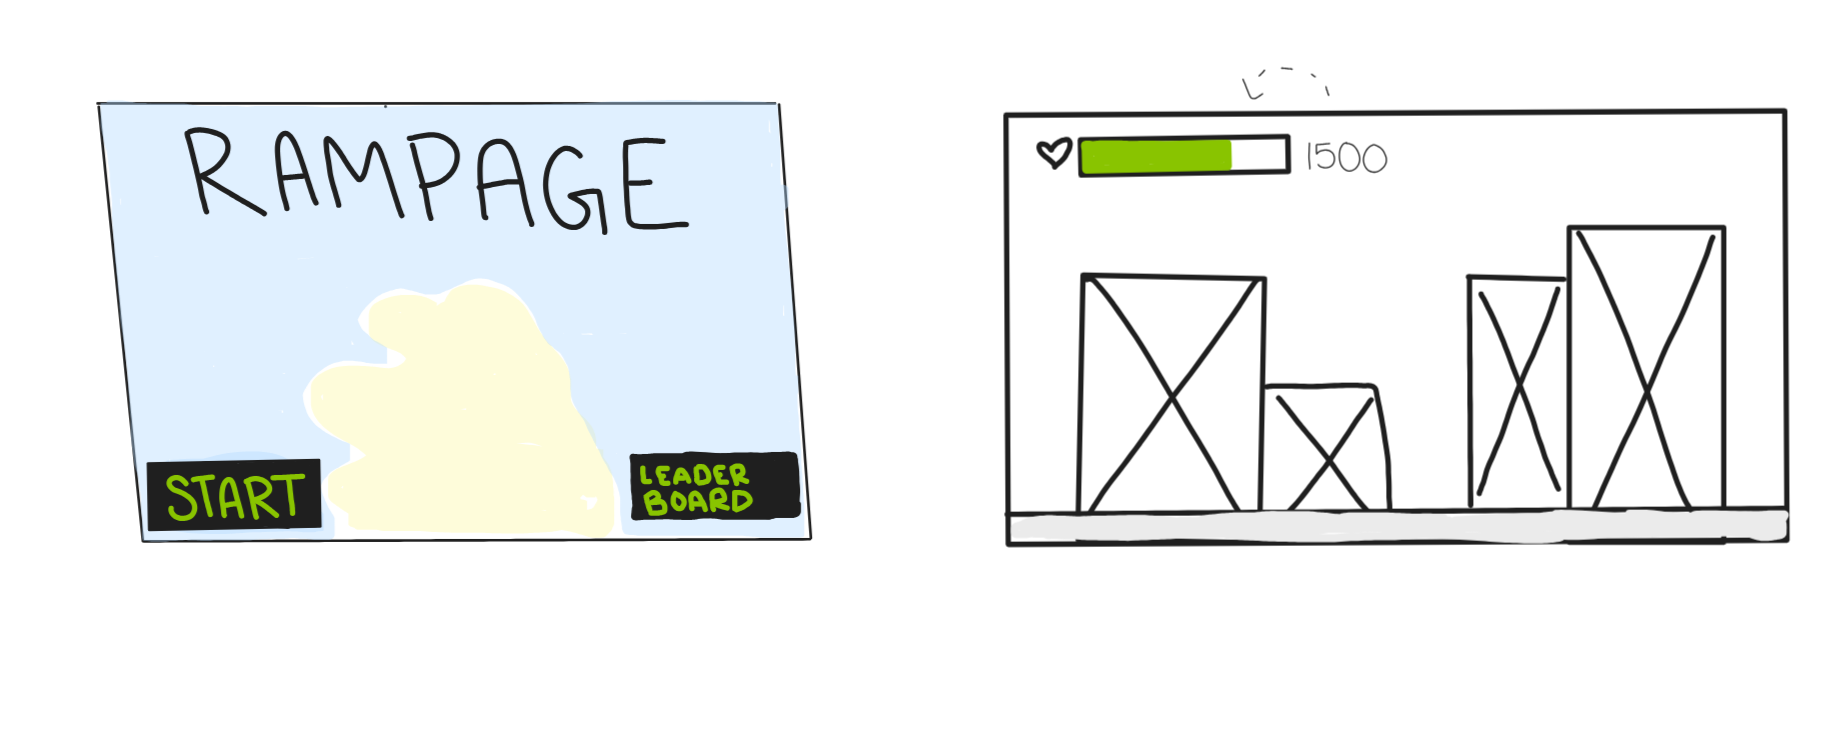
\includegraphics[width=1\textwidth]{diagrams/Wireframe.png}
    \caption{Image of wireframe.}
    \label{wireframe}
\end{figure}

\begin{figure}[h!]
    \centering
    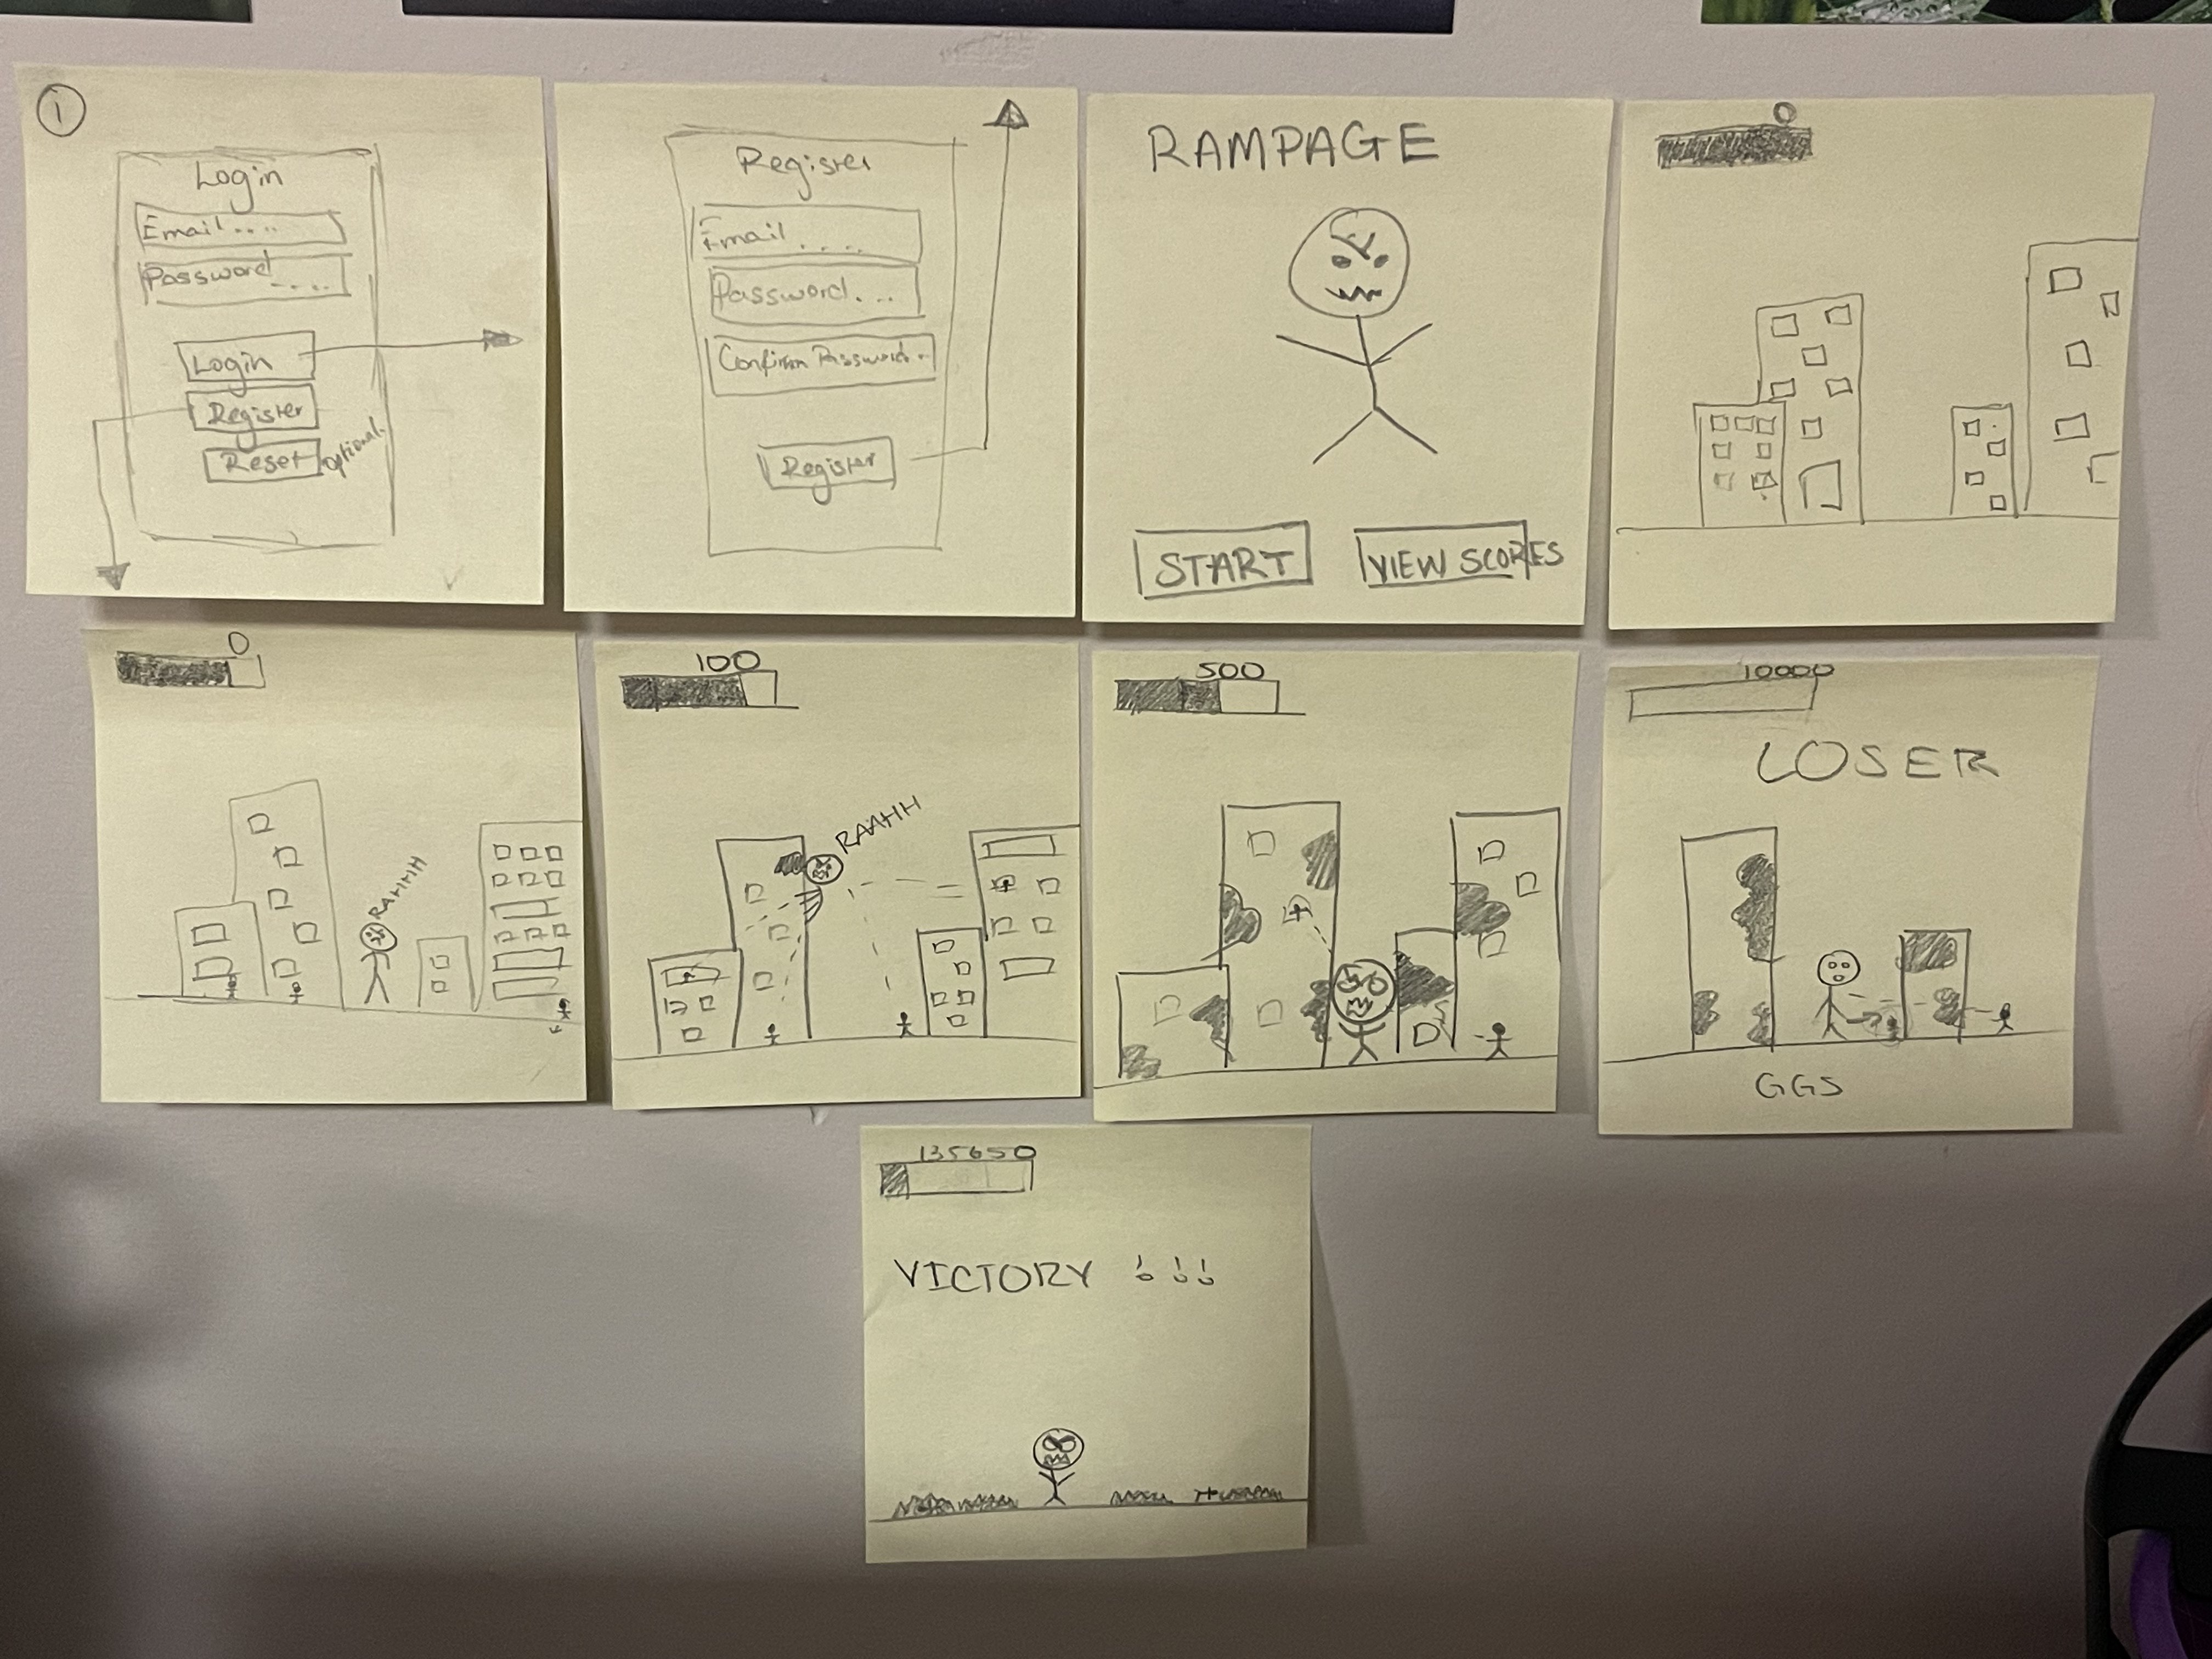
\includegraphics[width=1\textwidth]{diagrams/Storyboard.jpg}
    \caption{Image of storyboard.}
    \label{storyboard}
\end{figure}

%---------------------------End Wireframes and Storyboard----------------------------------

% No text here.

%---------------------------Unified Modeling Language----------------------------------
\subsection{UML}

\subsubsection{Class Diagrams}
%At least one for each design pattern category.   
%Each class diagram should include the following:
%	Title for each Class Diagram
%	Description of how and why each class is used
%	Mapping to source code (in the Appendix, specific files and line numbers) of where it’s used.
Enemy Prototype Diagram:
The enemies/NPCs have multiple character types like walkers, helicopters, and tanks. The most common function walkers and helicopters have is the ability to fire at the player with all enemies having the ability to spawn. 

Within our game, we have many NPCs that all share some forms of the same functionality including spawning and attacking the player. Using the prototype diagram helps us efficiently make the same methods that can go across the various types of NPCs. We have also included the civilian NPCs because although they do not necessarily harm the player’s character, they still have some of the same functionalities as a soldier. 


Game Objects Observer Diagram:
When recreating this game, we had many objects that we needed to monitor. We have many NPC objects and building objects that take various state changes during the gameplay, and we need to implement algorithms to take these state changes into consideration. The Observer diagram is the best behavioral diagram we could use for our game since we need to observe the state changes of the other objects outside of the player themselves. The methods can also stop affecting any object that does not need the method implemented on them at any time.

Player and Enemy Façade Diagram:
The more complex code is for both the players and the enemies. Scripts for the player and the enemies are made from even smaller codes behind a much bigger interface.

We chose to sketch out the façade diagram since we only recreated one level of Rampage. Our diagram depicts our façade class holding the startGame() method, and it illustrates how the other methods and objects interact with it. Overall, our Facade diagram promotes loose coupling between the player and the system by providing a simplified interface of the gameplay. It helps manage complexity and improves maintainability in large systems. 



%uncomment the section below when you're ready to insert an image
\begin{figure}[h!]
    \centering
    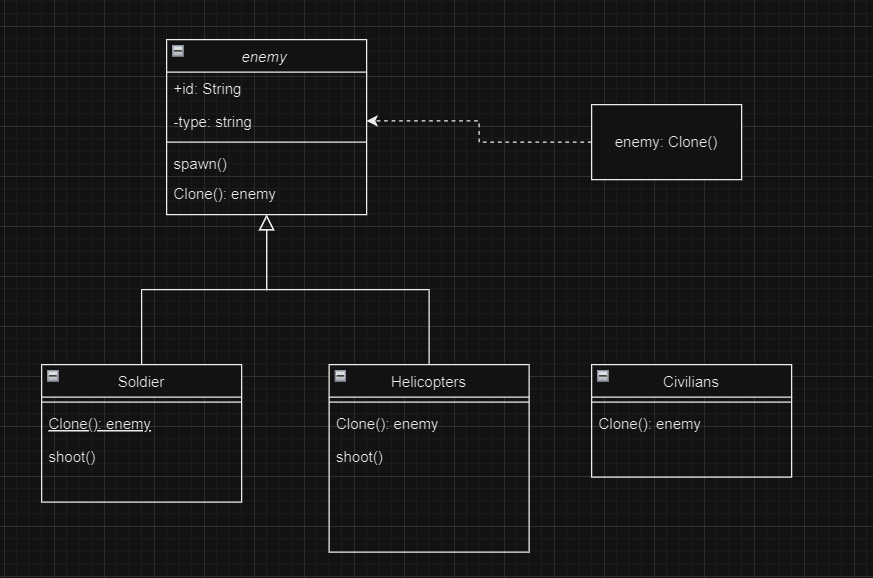
\includegraphics[width=1\textwidth]{diagrams/Prototype.png}
    \caption{Prototype diagram showing how most of our }
    \label{prototype_diagram}
\end{figure}


%uncomment the section below when you're ready to insert an image
\begin{figure}[h!]
    \centering
    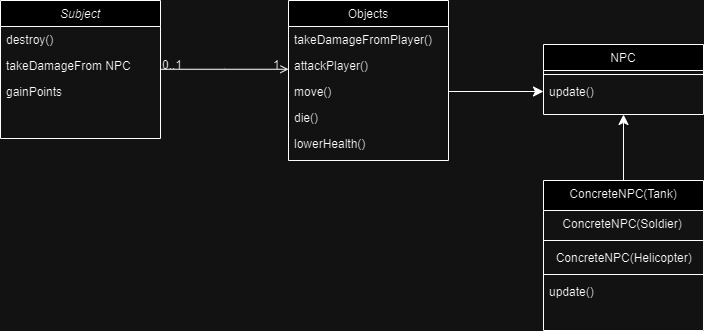
\includegraphics[width=1\textwidth]{diagrams/Observer.jpeg}
    \caption{Observer diagram shows }
    \label{observer_diagram}
\end{figure}


%uncomment the section below when you're ready to insert an image
\begin{figure}[h!]
    \centering
    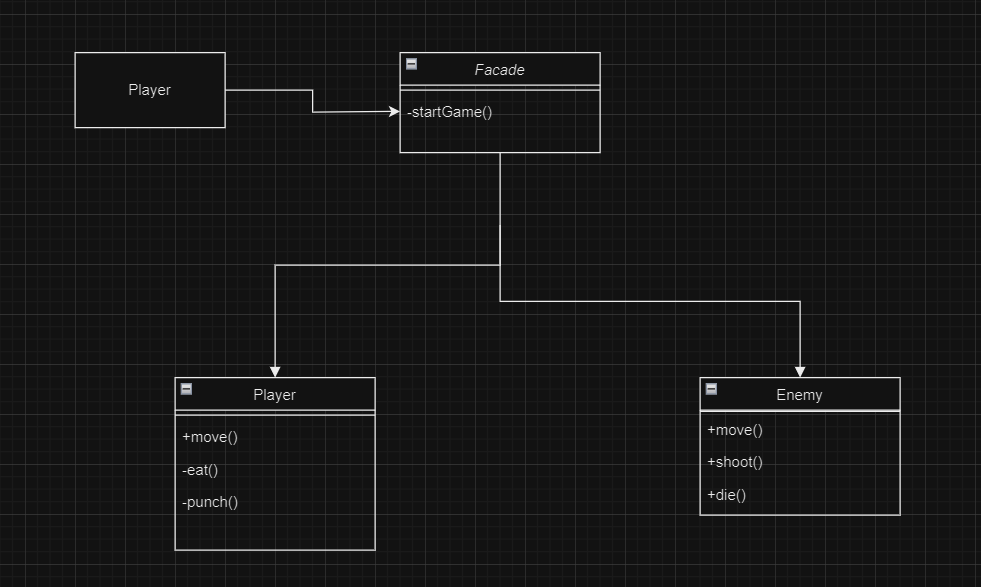
\includegraphics[width=1\textwidth]{diagrams/Facade.png}
    \caption{Façade diagram shows the relationship between the player and enemies.}
    \label{facade_diagram}
\end{figure}


\subsubsection{Use Case Diagrams}
%Enough to cover all technical functional requirements.
%Each Use Case Diagram should include the following:
%	Title for each Use Case Diagram
%	A description of information given in the diagram.
%	Mapping to source code (in the Appendix, specific files and line numbers) of where it’s used.
Title: Player Activity Use Case Diagram

The user is the player and when the game is booted up, they have two choices when on startup: to play or exit the game. When the player exits, it exits the game, but when you play the game, you must create a sign in, and you can choose one of three characters to play as. Once selected, you can use the keyboard to move and punch buildings. We decided on this layout because it was easier to describe what the user can do while playing the game. 


%uncomment the section below when you're ready to insert an image
\begin{figure}[h!]
    \centering
    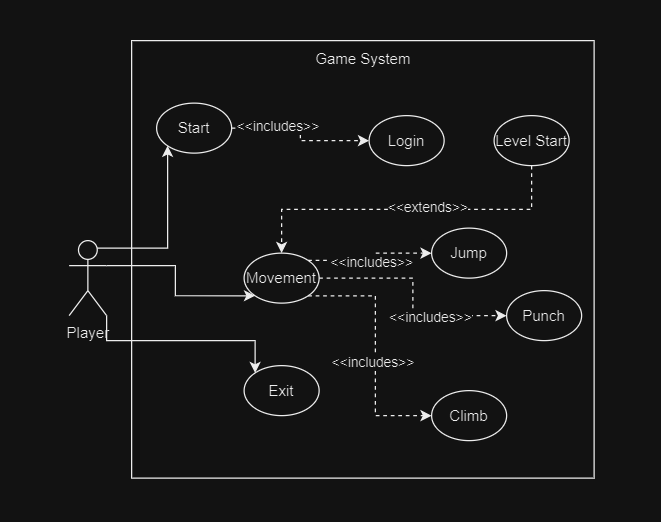
\includegraphics[width=1\textwidth]{diagrams/UseCaseDiagram1.png}
    \caption{Use case diagram showing the player interactions with the game.}
    \label{use_case_diagram}
\end{figure}


\subsubsection{Use Case Scenarios Developed from Use Case Diagrams (Primary, Secondary)}
%Should include at least one primary and zero to many secondary scenarios
%Each Use Case Scenario should include the following:
%	Title for each Use Case Scenario
%	A short description of the information given in the scenario.
%	Mapping to source code (in the Appendix, specific files and line numbers) of where it’s used
Primary Use Case Scenario: The user starts the game by selecting the “play game” option from the menu. The player can potentially select their character they can play as. The player then clicks advance, and the environment loads, including the buildings and NPCs. The player then gains control of the monster and they start moving around the environment using the keyboard. By doing so, they destroy buildings and gain points. The player also much avoid the soldiers, tanks and helicopters in order to live and destroy, thus collecting points. If the player completes the objective of destroying all the buildings, they win. If they don’t complete it by the time their health runs out, they lose. After the level is complete, the score is displayed.  

Secondary use case scenario: Occasionally, the player can get an alert indicating that the tanks and helicopters are approaching. The player must move the monster to avoid these new strikes. The player can also stomp on the tanks and punch the helicopters, destroying them and collecting points as well. After evading these attacks, the player resumes their task of destroying buildings.

%uncomment the section below when you're ready to insert an image
\begin{figure}[h!]
    \centering
    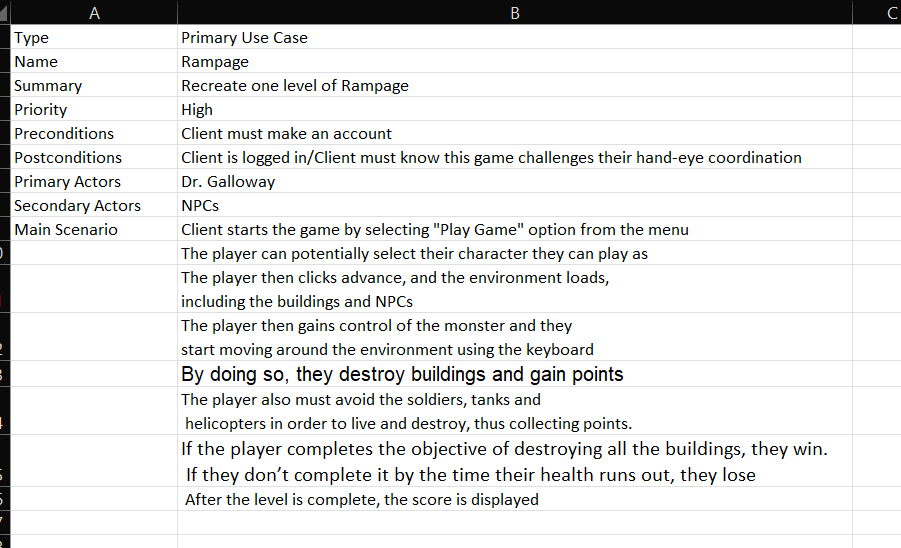
\includegraphics[width=1\textwidth]{diagrams/PrimaryUseCaseScenario.png}
    \caption{Use Case Scenario 1}
    \label{use_case_scenario}
\end{figure}


%uncomment the section below when you're ready to insert an image
\begin{figure}[h!]
    \centering
    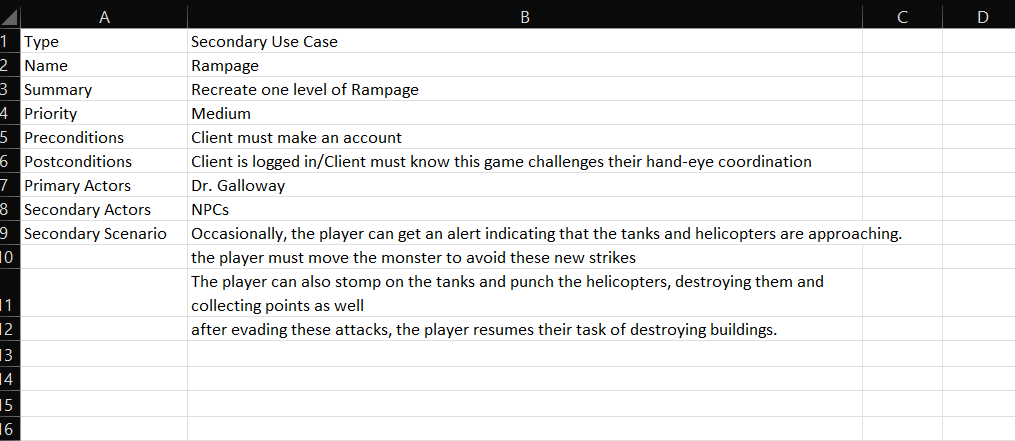
\includegraphics[width=1\textwidth]{diagrams/SecondaryUseCaseScenario.png}
    \caption{Use Case Scenario 2}
    \label{use_case_scenario}
\end{figure}


\subsubsection{Sequence Diagrams}
%Each diagram should include all actors/resources to cover one Use Case Scenario.
%	Each Sequence Diagram should include the following:
%	Title for each Sequence Diagram
%	A short description of the information given in the diagram.
%	Mapping to source code (in the Appendix, specific files and line numbers) of where it’s used
Title: Game System Interaction Sequence Diagram

The diagram shows our overall game approach on interacting with the game system. First, once the user opens the game, the game shows the user a login prompt as well as the top scores which it will take from the database that we will use for this project. Once the user logs in, the game system will check the database to verify that the user exists within it. If the login credentials are valid, the database notifies the game system and the user is able to start playing the game. Within the gameplay, the enemy npcs will target the user and the user can kill npcs and destroy buildings. Once all buildings are destroyed, the game notifies the user that the level was completed and shows their score. The user cam then save those scores, which will be saved to the database.

%uncomment the section below when you're ready to insert an image
\begin{figure}[h!]
    \centering
    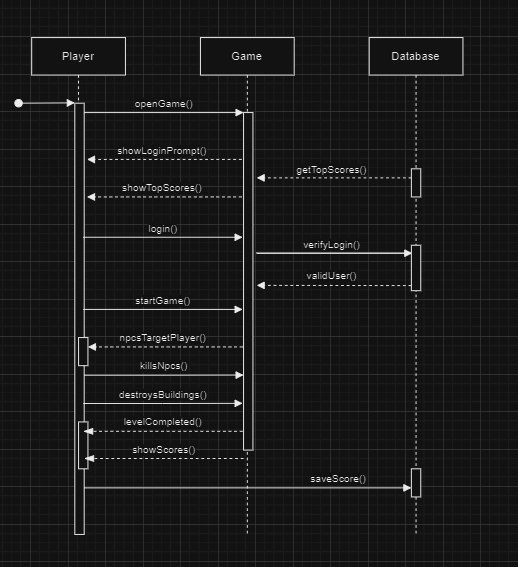
\includegraphics[width=1\textwidth]{diagrams/Sequence1.png}
    \caption{Sequence diagram on the overall software function.}
    \label{sequence_diagram}
\end{figure}

\subsubsection{State Diagrams}
%Each diagram should identify the object/resource/asset (in the title of the diagram) and display all states and actions/events that create state changes.
%	Each State Diagram should include the following:
%	Title for each State Diagram
%	A short description of the information given in the diagram
%	Mapping to source code (in the Appendix, specific files and line numbers) of where it’s used
Title: Game System State Diagram

When the user starts the game, the game is in the starting state. When the user hits pause, the game goes into a paused state. When the user presses resume, the game goes back to its starting state. If the player dies or completes the level, the game goes into an end state and the player has the option of restarting the level which would put the game back into its starting state.

%uncomment the section below when you're ready to insert an image
\begin{figure}[h!]
    \centering
    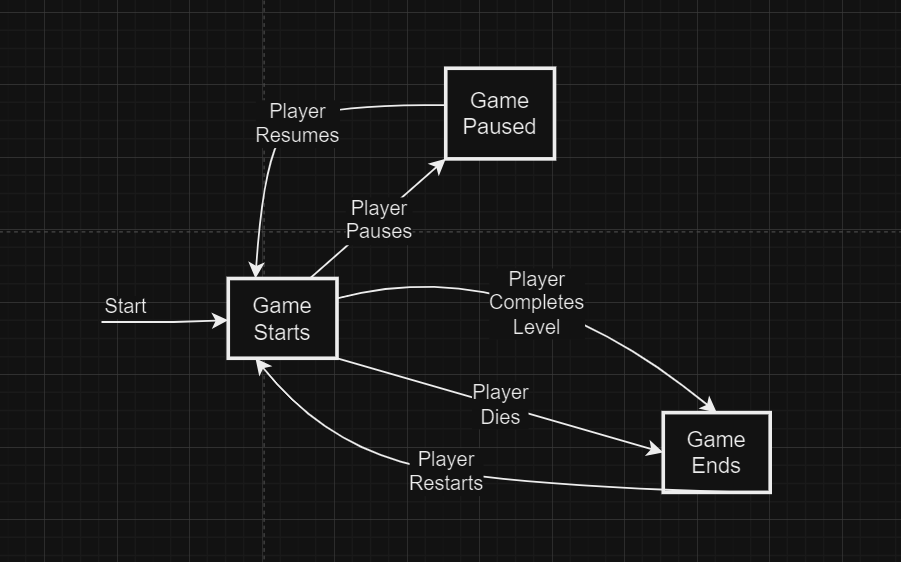
\includegraphics[width=1\textwidth]{diagrams/StateDiagram.png}
    \caption{State diagram on the overall game state.}
    \label{state_diagram}
\end{figure}

\subsubsection{Component Diagrams}
%Single diagram that defines component APIs and communication pathways for all software and dependencies used in the product.
%	The Component Diagram should include the following:
%	Title for the Component Diagram
%	A description of the information given in the diagram
%	Protocols used for each communication pathway
%	Mapping to all source code and dependency software (in the Appendix, specific files)
Title: Game Aspects Component Diagram

This diagram shows that each aspect of our game feeds into Unity and its interface(s). The game tools, which includes key controls and pause menu screens; the game contents, such as audio, graphics, settings, and the network; then the game utility, which contains the logging system and math utilities and libraries. All three of those things feed into the game engine. 

%uncomment the section below when you're ready to insert an image
\begin{figure}[h!]
    \centering
    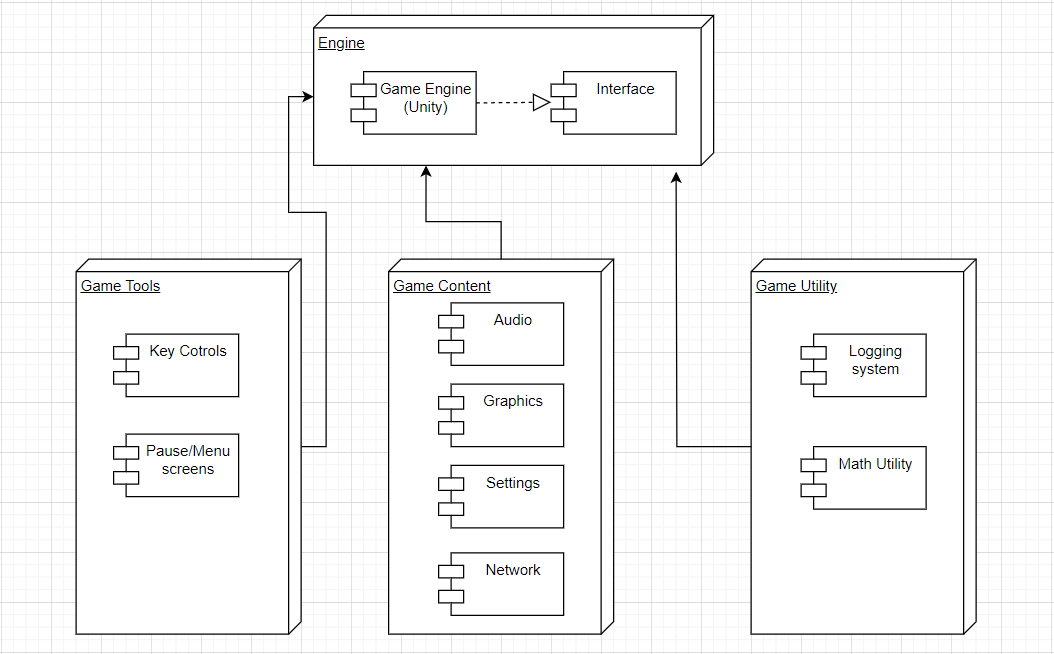
\includegraphics[width=1\textwidth]{diagrams/Component.png}
    \caption{Component diagram showing the how aspects of our game feeds into Unity and interfaces.}
    \label{component_diagram}
\end{figure}

\subsubsection{Deployment Diagrams}
%Single diagram that defines the physical nodes, virtual nodes, and communication for all software related to the product.  Should be an extension of the Component Diagram.
%	The Deployment Diagram should include the following:
%	Title for the Deployment Diagram
%	A description of the information given in the diagram
%	Identify all physical and virtual nodes used for process execution
%	Identify all internal and external node communication
Title: Game File Deployment Diagram

The deployment diagram shows that the game file containing all unity files, scripts, and assets is contained within Unity - which the user will use to play the game. All of this is occurring on the user’s computer/PC. There is no outside server or connection to someone else’s server or computer.

%uncomment the section below when you're ready to insert an image
\begin{figure}[h!]
    \centering
    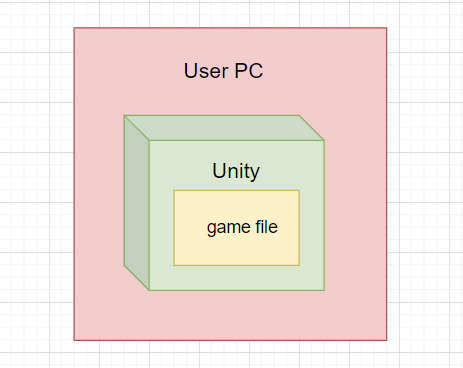
\includegraphics[width=1\textwidth]{diagrams/Deployment.png}
    \caption{Deployment diagram showing how our game is deployed.}
    \label{deployment_diagram}
\end{figure}

\subsection{Traceability Table}

%\begin{table}[h!]
%\centering
%\begin{tabular}{lllll}
%\hline
%\textbf{ID} & \textbf{Description} & \textbf{Purpose} & \textbf{Dependencies} & \textbf{Status} \\ \hline
 %1 & Character & Gameplay & N/A  & Not started  \\ \hline
% 2 & Building & Gameplay & Player & Not started  \\ \hline
% 3 & Tank & Gameplay & Player, pathfinding & Not started  \\ \hline
 %4 & Soldier & Gameplay & Player, pathfinding & Not started  \\ \hline
 %5 & Airplane & Gameplay & Player, pathfinding & Not started  \\ \hline
% 6 & Tower & Gameplay & Player, pathfinding & Not started  \\ \hline
% 7 & Explosion Effect & Aesthetics & N/A & Not started  \\ \hline
% 8 & Street & Aesthetics & Lighting & Not started  \\ \hline
% 9 & Background & Aesthetics & Lighting & Not started  \\ \hline
%\end{tabular}
%\end{table}


\begin{figure}[h!]
    \centering
    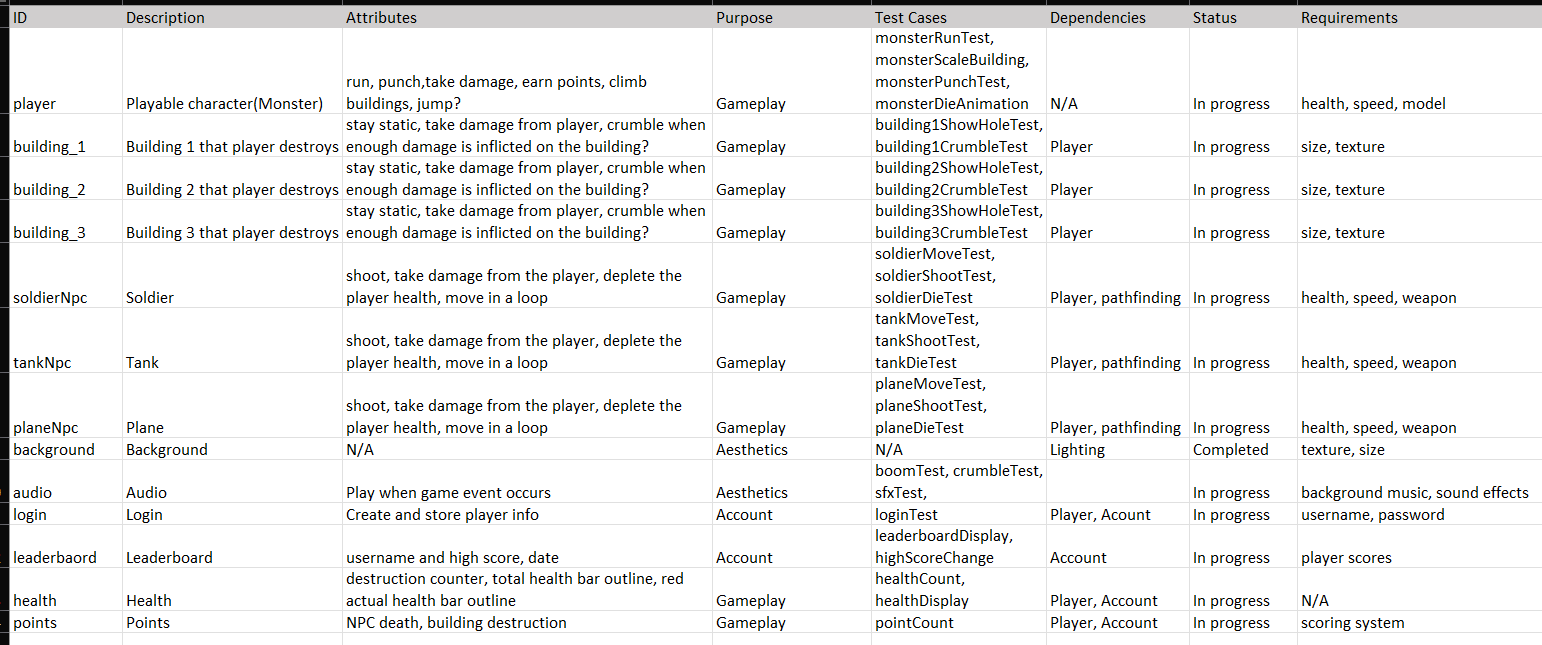
\includegraphics[width=1\textwidth]{diagrams/TraceabilityTable.png}
    \caption{Requirements Traceability Table.}
    \label{traceability_table}
\end{figure}

The following traceability table outlines the many components of our recreation of Rampage. Each row represents a specific element that is categorized by its characteristics and  status in terms of development. 

This table helps us track the progress of all of these aspects of the Rampage development process. It indicates which components fall under the categories of Gameplay and Aesthetics, lists any dependencies required for each component, and provides an update on their current status. At the time of project completion, all sections should be completed.

%---------------------------End Unified Modeling Language----------------------------------

% No text here.

%---------------------------Version Control------------------------------------------------
\subsection{Version Control}
%200 words minimum
%Describe your group's approach to version control.  Include details on how and when you make commits to GitHub.  Explain version naming, branching, and integration approaches.
Version control was a big unknown when we had started this project. We were in between on using Google Drive and GitHub though we had never used GitHub before. We knew that Google Drive would have a lot of issues with syncing changes with other team members and by only supporting one member making changes at a time, so GitHub seemed like a better alternative. Though GitHub has a lot of issues of its own, we have been managing with it and learned how to somewhat use it correctly. After learning the basic way of syncing GitHub with Unity from a YouTube video, the only problem we had was that sometimes committed changes took awhile to show up on another member’s laptop after pulling from origin. 

We usually made commit changes to the repository after we had completed a big section of our task for the project or when we were done working on it momentarily. We named our commits based on what we were working on or had completed in those changes. We used the GitHub desktop that is connected to the repository, and create changes through that. We all worked on the same branch, the main branch, to make commits. This may have been the issue to an earlier problem that we had faced but it all sorted itself out without intervention. 



%---------------------------End Version Control------------------------------------------------

% No text here.

%---------------------------Data Dictionary------------------------------------------------
\subsection{Data Dictionary}
%200 words minimum and table
%	Create a table that displays your Data Dictionary and describe how it is being used to define data structures and other major variables/elements in the software product.
The following data dictionary provides a comprehensive overview of the game elements and mechanics for the recreation of our level in the game Rampage. This table is categorized in game objects, collisions, game mechanics, user interface and audio. The monster, soldierNPC, tankNPC, planeNPC, building1, building2, building3 and background are categorized as game objects. The monster is a playable character whose role is to destroy the entire city. The soldierNPC, tankNPC and the planeNPC are the nonplayable characters whose purpose are to defend the city from the monster. building1, building2, building3 are the city buildings that the monster destroys and the city that the military are trying to protect. The background city scene’s purpose is to enhance the visual experience of the game. The elements incorporated in the collision category are playerClimbBuilding, playerPunchBuilding, npcShootPlayer, and playerKillNPC. The playerClimbBuilding and playerPunchBuilding collisions define the interactions between the player and buildings using a box collider. The npcShootPlayer and the playerKillNPC collisions define the interactions between NPCs and the players using capsule colliders. The scoring rules, winning conditions and losing conditions are incorporated into the game mechanics. The scoring rules are that the players earn points for specific actions, such as eating soldiers, squishing tanks and planes, and damaging buildings. The winning conditions are to destroy all the buildings while still maintaining enough health to survive. The losing conditions are to die before destroying the entire city. The user interface(HUD) contains the following aspects: health bar background, health bar fill and points. The health bar background represents the initial total health that remains static at the start and as the player’s health depletes. The health bar fill indicated the player’s current health. It decreases as the player takes damage. The points element tracks points earned by the monster player through actions like city destruction and defeating military forces. Within the audio category, there are two elements: sound effects and the theme song. The sound effects are various sound effects like “boom” for explosions. The theme song plays in the backgrounf for entertainment purposes, independent of the game functionality. 


%uncomment the section below when you're ready to insert an image
\begin{figure}[h!]
    \centering
    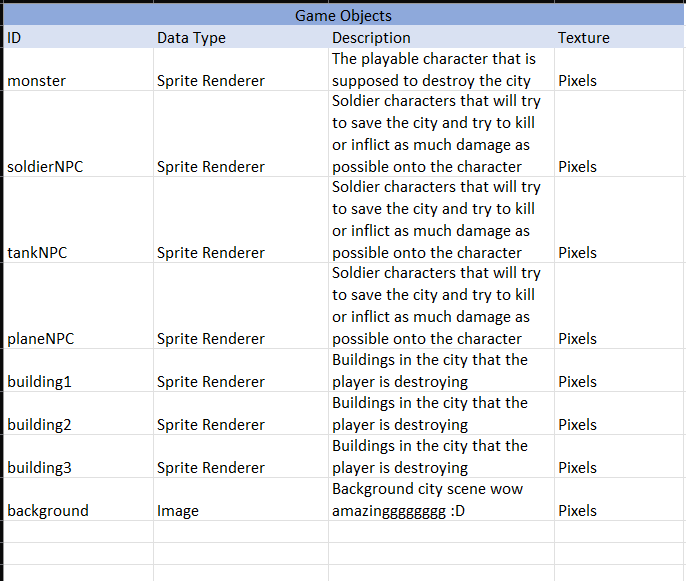
\includegraphics[width=1\textwidth]{diagrams/DataDictionary1.png}
    \caption{Data dictionary table game objects.}
    \label{data_dictionary}
\end{figure}

\begin{figure}[h!]
    \centering
    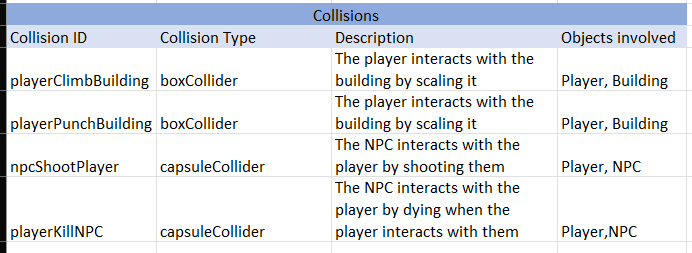
\includegraphics[width=1\textwidth]{diagrams/DataDictionary2.png}
    \caption{Data dictionary table collisions.}
    \label{data_dictionary}
\end{figure}

\begin{figure}[h!]
    \centering
    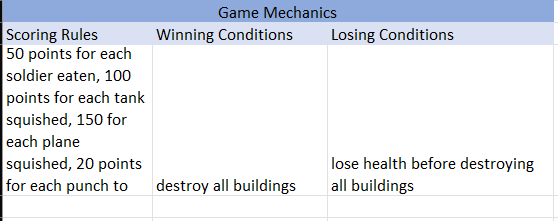
\includegraphics[width=1\textwidth]{diagrams/DataDictionary3.png}
    \caption{Data dictionary table game mechanics.}
    \label{data_dictionary}
\end{figure}

\begin{figure}[h!]
    \centering
    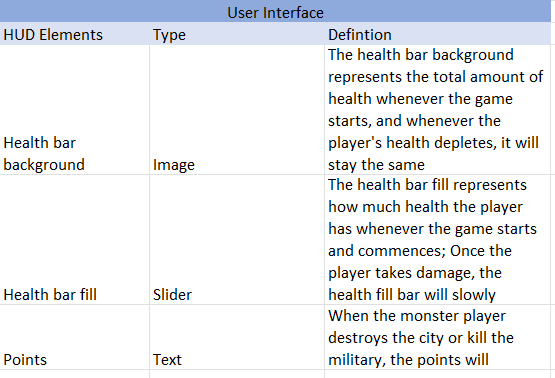
\includegraphics[width=1\textwidth]{diagrams/DataDictionary4.png}
    \caption{Data dictionary table user interface.}
    \label{data_dictionary}
\end{figure}

\begin{figure}[h!]
    \centering
    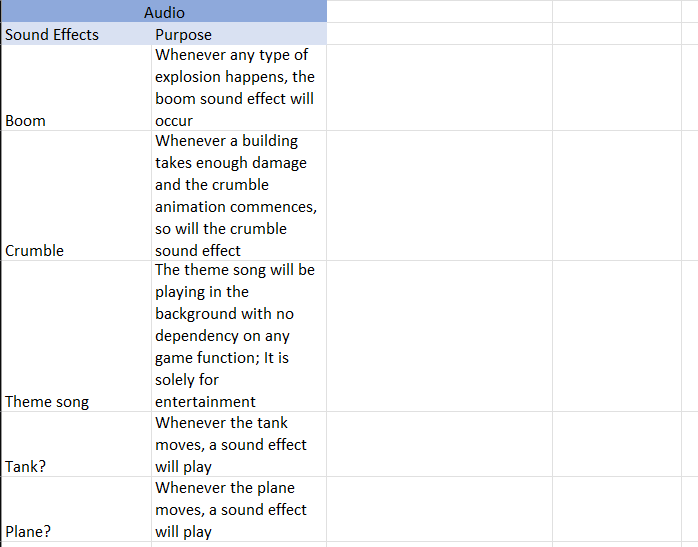
\includegraphics[width=1\textwidth]{diagrams/DataDictionary5.png}
    \caption{Data dictionary table audio.}
    \label{data_dictionary}
\end{figure}


%---------------------------End Data Dictionary------------------------------------------------


% No text here.

%---------------------------User Experience Details------------------------------------------------
\subsection{User Experience}

\subsubsection{Gameplay Diagram}
%150 words minimum
%Also called a controlled flow graph.  Insert an image of the gameplay diagram and describe the diagram in detail.
This diagram illustrates the flow of how our game should operate. The user will start the game up. They are then asked to login, if they do not have an account, they will create one and then login. Once they have done that, they will then have the option to start the game or look at the leaderboard. Clicking the leaderboard option will show the leaderboard and then lead the player back to the menu. The player clicks start and then the gamplay begins. They will play a character that destroys buildings, which earns them points as the buildings take damage. They will be attacked by NPCs, which will gradually deplete their health. If the player’s health bar reaches zero, they will die and lose the game. However, the player can attack NPCs. When they attack, the NPCs lose health and die. If the player gets enough points and their health bar is not empty then they win and the game is over.

%uncomment the section below when you're ready to insert an image
\begin{figure}[h!]
    \centering
    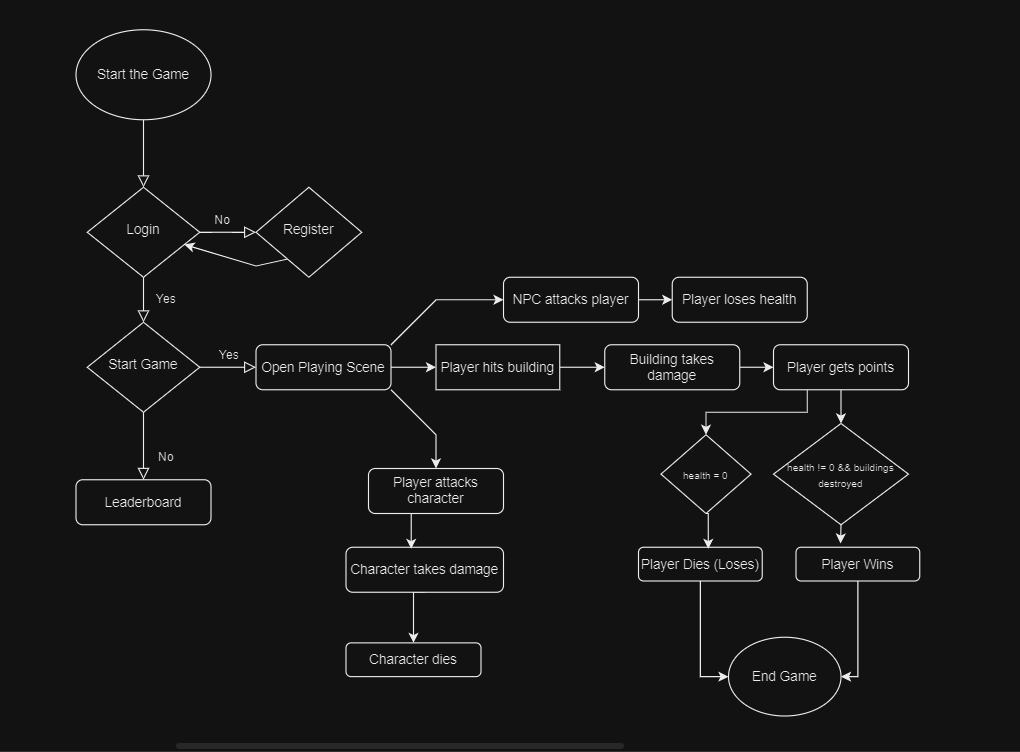
\includegraphics[width=1\textwidth]{diagrams/GameplayDiagram.png}
    \caption{Diagram of Rampage Gameplay.}
    \label{gameplay_diagram}
\end{figure}

\subsubsection{Gameplay Objectives}
%150 words minimum
%Should explain why someone should play your game. Should define the goals of your game.
Our game challenges hand-eye coordination and strategy. The player must be able to make the moves they decide on quickly and efficiently using their keyboard. They also need to be able to strategize and think on the fly. They need to strategize how to destroy the buildings without coming into contact with the NPCs near them. If they come into contact with an NPC, they lose a life so they need to avoid them as much as they possibly can. Playing this game will keep their intellect and reflexes sharp as they move throughout the game and destroy the buildings in order to gain all available points without losing all of their lives in their efforts.


\subsubsection{User Skillset}
%150 words minimum
%Describe the abilities a user should have in order to interact with the software: Screen tapping, Memorization, Puzzle, solving, Strategy development, Quick reflexes 
The user is able to interact with the game by using their mouse or trackpad and a keyboard. There is no screen interaction capability, so the user will not be able to use a digital touchscreen keyboard – it must be physical. Even if the game supported screen interaction, a digital keyboard when get in the way of the game presentation on the screen and interfere with the gameplay. There is no memorization or puzzle solving, but they need to develop strategies as they play and use quick reflexes to avoid losing their lives coming into contact with enemies. The user needs to have some level of muscle memory and know how to type without having to reference the keyboard. They will need to be able to control the keys without taking their eyes off of the screen so that they can still notice and react to enemy NPCs and changes in health and score while they play.


\subsubsection{Gameplay mechanics}
%150 words minimum
%Thorough guide of the game rules: Turn-based, Random chances, Capturing/eliminating, Time-based, Team-based
This game is a point-based game. The user is trying to achieve 100,000 points to win. There is no time limit, however if their lives depletes to zero they lose; they only have three lives. The rules are as such: the player can destroy buildings by finding the collision boxes built into them. They do this by jumping around the building. The entire time they must avoid enemies. There is no way to replenish lost lives. The user can move to the enemy and jump on them to kill them – but coming into contact with them will still take a life so they must use this strategically. There is not multi-player funcitonailty so they cannot team up with someone to divide and conquer or race against. It is simply them vs. the enemies until they either destroy all of the buildings or lose all of their lives.


\subsubsection{Gameplay Items}
%150 words minimum
%This section of the GDD refers to smaller elements of the game, such as: Health/power-ups, Coins, Loot crates, Weapons/character upgrades, Etc. Changes gameplay elements as the player progresses through the game.
The user does not encounter any health tokens or powerups in our game. There are no coins, loot, or character upgrades that can be made. The user remains as the main character, George, in his one state of being for the entirety of the game. George does not have any powers or special abilities. He can walk, jump, climb buildings, punch, and squash soldiers. That is all that the user is able to do as they play through the game. If we continue this project in the future and add other levels, George could get 2x points for 30 seconds or something of a similar effect, however, that is out of our scope we have created for this project as we are simply recreating the first introductory level of the game. There are no special tricks, especially not any that would have any effect on the gameplay.

\subsubsection{Gameplay Challenges}
%150 words minimum
%Description of game challenges as a player progresses. Identify how a player handles difficulties and ensures the player can obtain essential tools to continue progressing through the game.
The player has everything they need to win the second they start the game. George does not need any special abilities, he simply needs to be able to move around, destroy buildings, and squash enemies. This makes it simple enough for someone with a lower skillset to be able to enjoy playing, but something with a higher skillset could replay as many times as they want to make improvements to their score. They would know, however, that any improvements they see are a reflection of the improvement of their hand-eye coordination or their strategy; it shows personal improvement, not an easier win with assistance. They are not given a helping hand when they encounter difficulties, which forces them to be involved and strategize as they play to be able to win and potentially increase their score each time. A spot on the leaderboard would be earned through their practice work, not a gift from the game.


\subsubsection{Gameplay Menu Screens}
%150 words minimum and wireframes
%Game start menu screen, pause menu screen, game over screen
%Give wireframe/drawing/image for all menus in the game.
The first screen the user sees when they open the game is the login screen. If they already have an account, they can just go ahead and login. If they need an account however, they can fill in their email and password in that login screen and hit "Register and Login" and their account has been created. Once they login, they see the main menu screen. Once here, they see two options. Option one is to see the leaderboard, which takes them to the leaderboard scene and then they  come back to the main menu. The second option is to start the game, which takes them into the game. Once the game is over, they will see either a win screen with a congratulatory message via audio, or they will see a lose screen that declares that they are, in fact, a loser. Both end case screens show "Game Over" and instruct the user on how to either play again, or logout. Screenshots of screens we have completed are attached.

%uncomment the section below when you're ready to insert an image
\begin{figure}[h!]
    \centering
    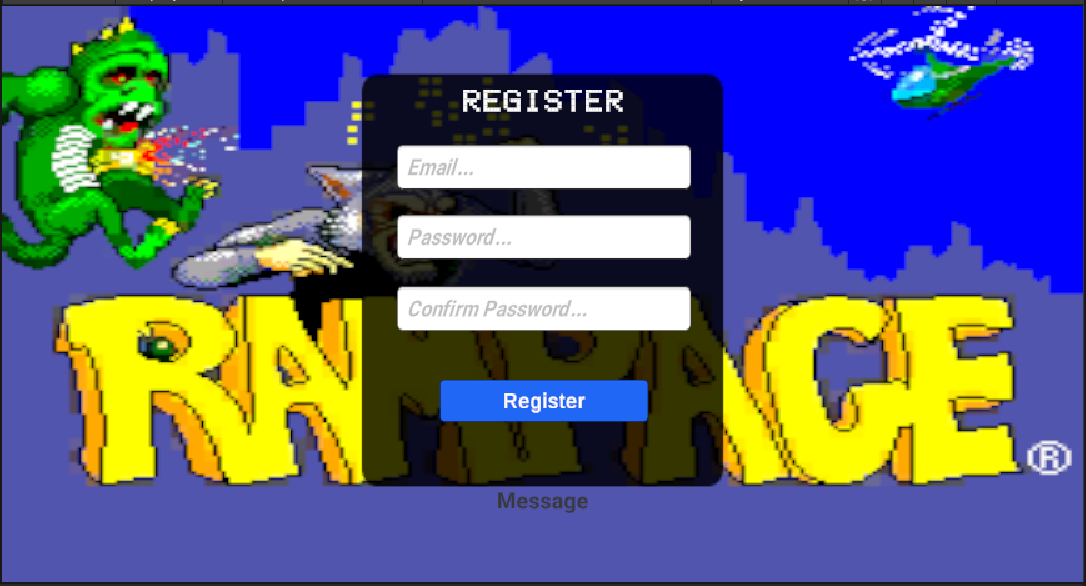
\includegraphics[width=1\textwidth]{diagrams/RegisterScreen.png}
    \caption{Image of Register Screen.}
    \label{register_screen}
\end{figure}

%uncomment the section below when you're ready to insert an image
\begin{figure}[h!]
    \centering
    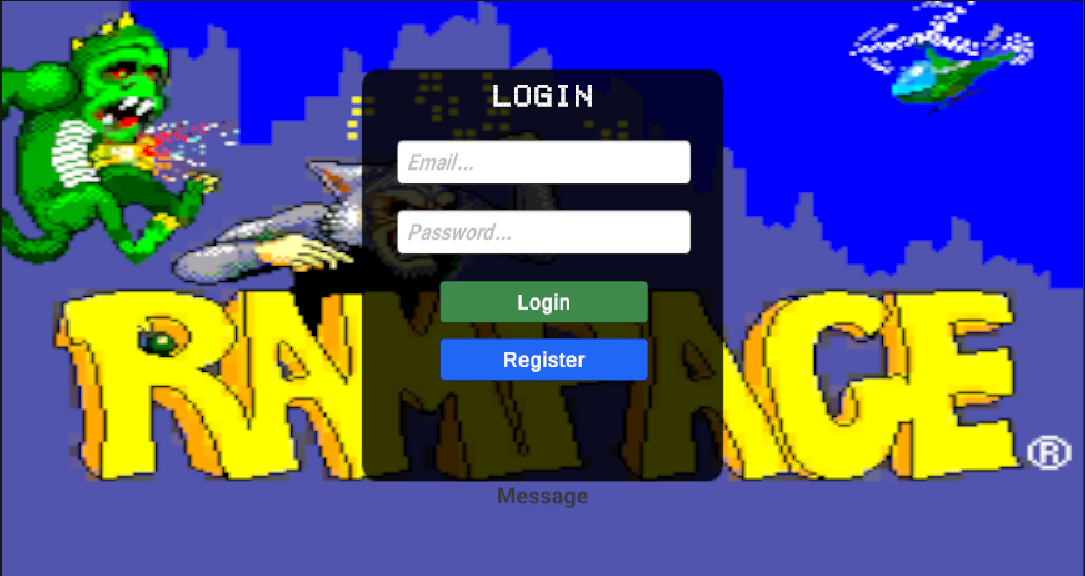
\includegraphics[width=1\textwidth]{diagrams/LoginScreen.png}
    \caption{Image of Login Screen.}
    \label{login_screen}
\end{figure}

%uncomment the section below when you're ready to insert an image
\begin{figure}[h!]
    \centering
    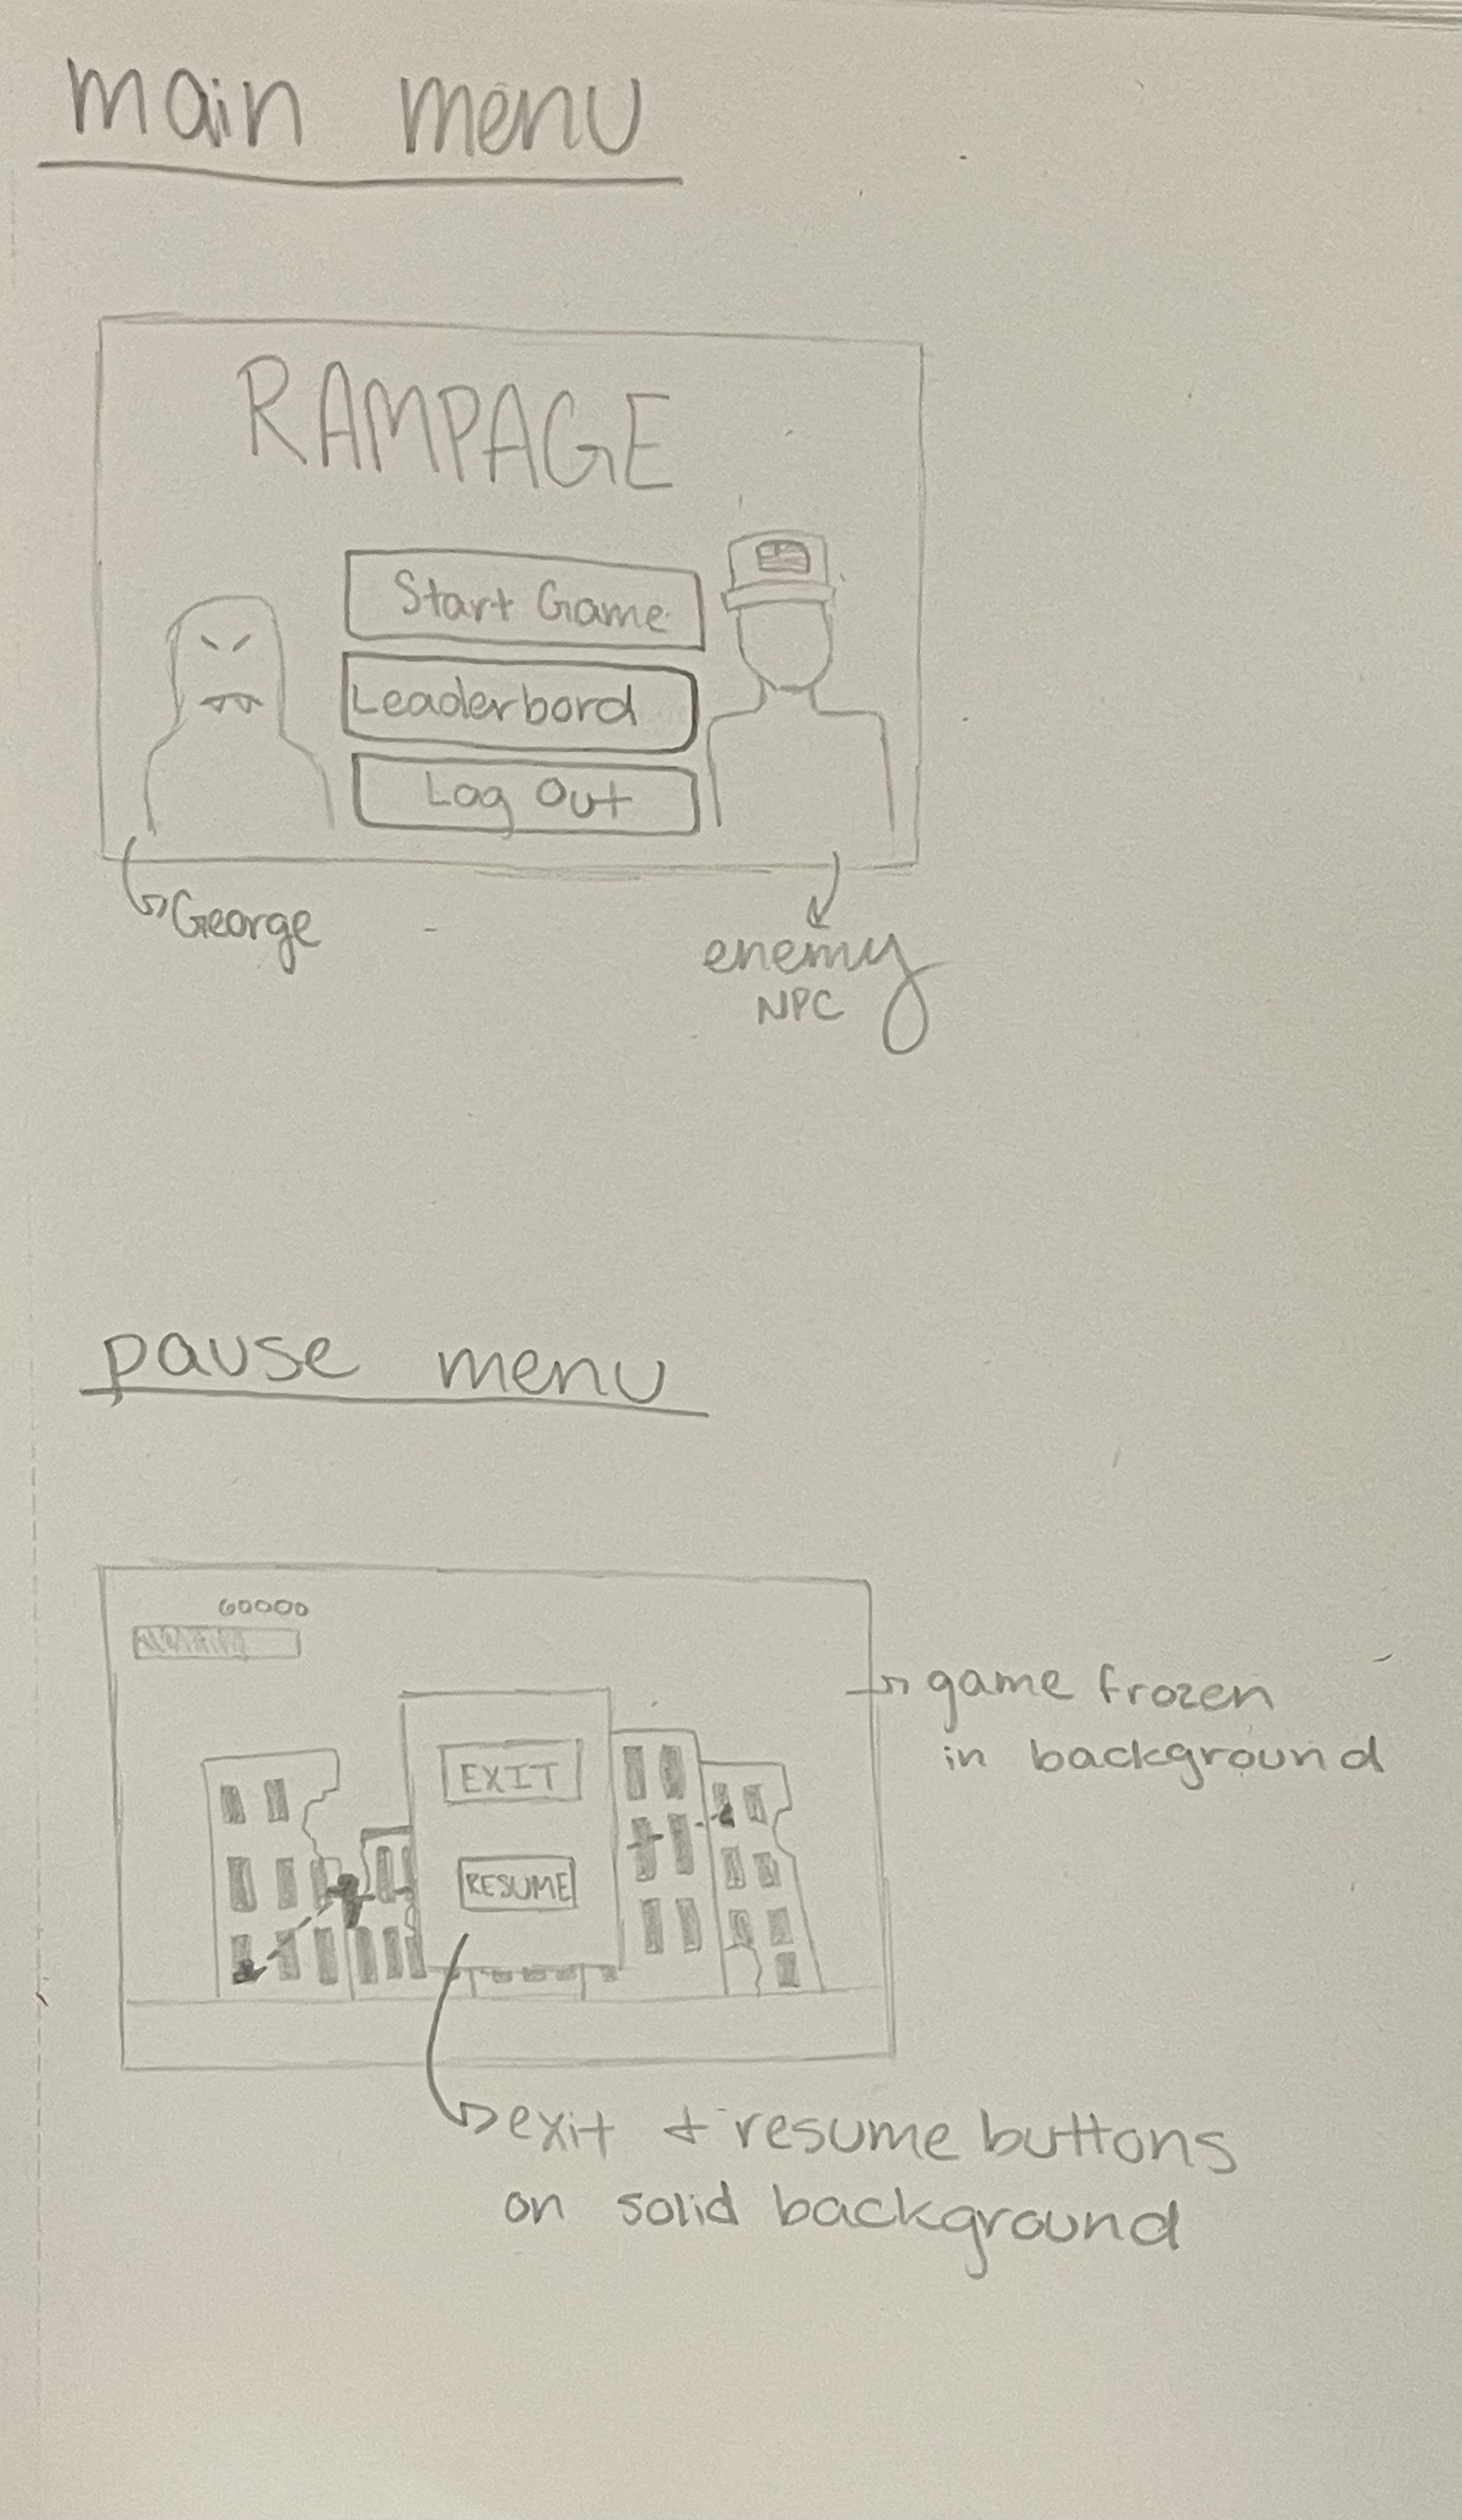
\includegraphics[width=1\textwidth]{diagrams/Menus.jpg}
    \caption{Image of Pause and Main Menus.}
    \label{pause_main_menus}
\end{figure}

%uncomment the section below when you're ready to insert an image
\begin{figure}[h!]
    \centering
    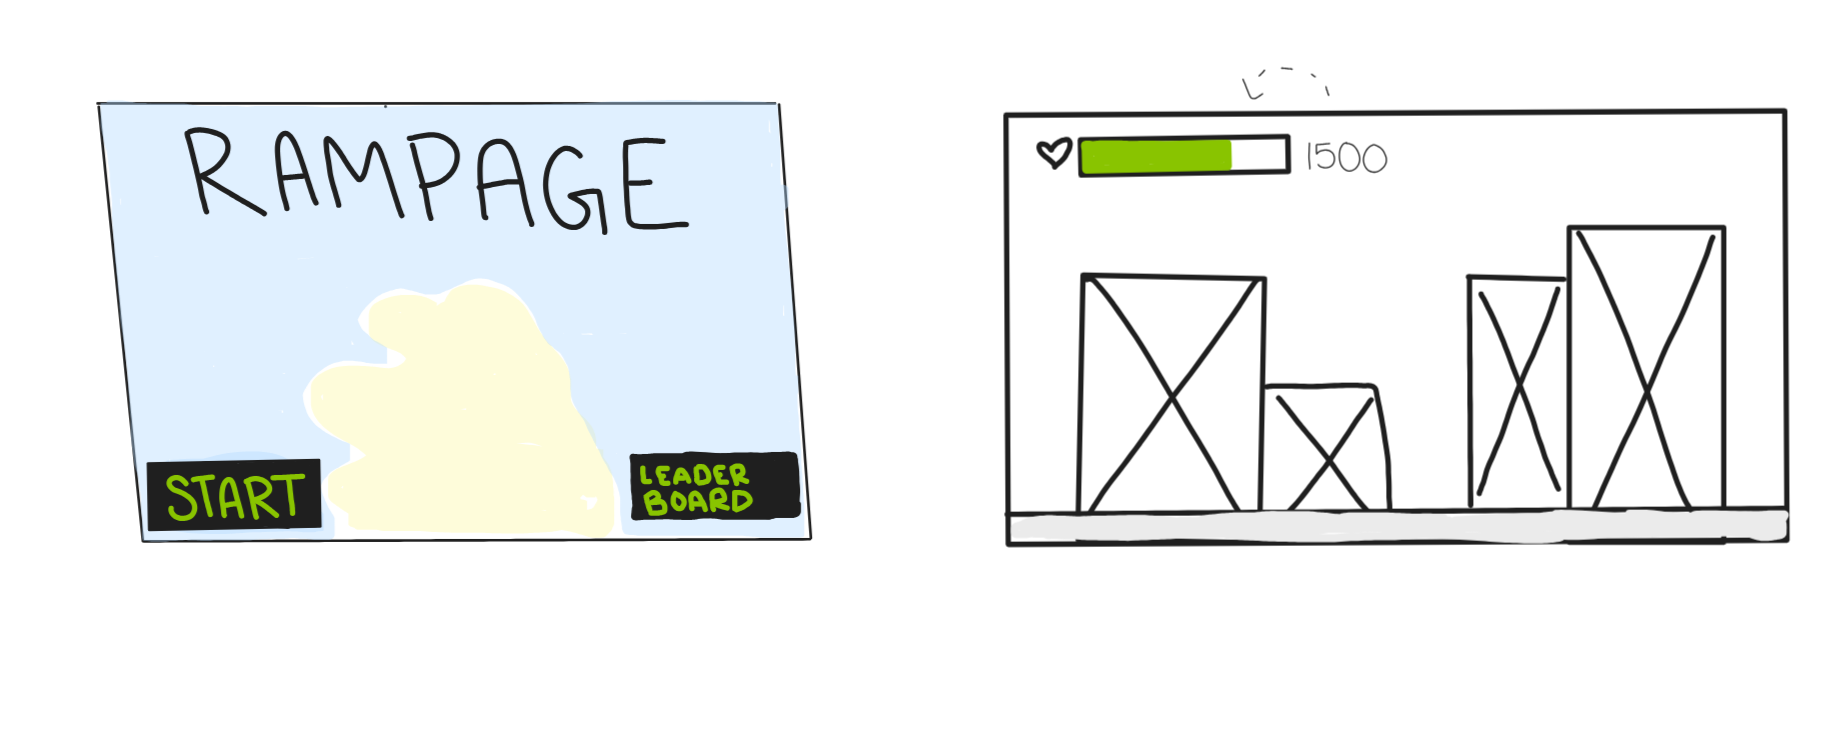
\includegraphics[width=1\textwidth]{diagrams/Wireframes.png}
    \caption{Images of the wireframes for main menu and gameplay.}
    \label{wireframes}
\end{figure}

\subsubsection{Gameplay Heads-Up Display}
%150 words minimum and wireframes
%Current Game information visually relayed to the player as a part of the game’s user interface.
%HUD features are generally static, on-screen so they remain visible during gameplay. Health/Lives, Time, Weapons/Ammo, Capabilities, Menus, Mini-Map, Score, etc.
Our heads up display is extremely simple. The user sees their score in the top left corner of their screen. If the score hits three, they win the game. The player sees their lives in the upper right hand corner. The lives start at three and count down each time they come into contact with an enemy NPC. These are texts that stay on screen throughout gameplay; there are no images, bars, or hearts implemented within our heads up display. Our player does not have any ammo or maps, so we do not need to implement any kind of visual in the heads up display for that. We do not need a map because our screen does not move – they see the same display on their screen for the entire game and they are unable to move away from that. Thus, no map is needed.

\subsubsection{Gameplay Art Style}
%100 words minimum
%describe the visual appearance of characters, objects, and other in-game elements. (Realistic, Cartoon, etc.)
Our game is a 2D cartoon pixelated style based off the visuals of games in the 1980’s. The characters are basic with very little detail – we were not trying for any kind of realism here. There is no depth, as it is 2D, so depth is implied by shadowed pixels in certain areas. The enemy NPCs will be basic pixelated drawings of soldiers. George himself is simple ape, and doesn’t rotate - he just moves side to side and jumps. There are simple animations for walking and jumping, and he flips when the player walks in different directions.


\subsubsection{Gameplay Audio}
%150 words minimum
%Description of all game audio: Character sound/voices, Ambient world sounds, Background music, etc.
Originally, we had set out to use gameplay audio that was accurate to the original game in the eighties. However, our client gave us permission to use custom audio in our game. Our background music is two of our members humming and beatboxing together. There are gun sounds eminating from the soldiers. The win and lose scenes contain a cappella music pertaining to either winning or losing done by one member and someone outside of the group. Each member also did various ambient sounds like buildings breaking and gun ‘pew’s. These audios were attached to the appropriate sprites and scripts for each scenario, and layer with each other well when needed. These audios were created/recorded on Andrea's phone and compiled into a folder for the game to utilize. They are mp3 files, and well labeled so that there is no confusion on which sound belongs to which aspect of the game. 



%---------------------------End User Experience Details------------------------------------------------

% No text here.


%---------------------------End Modeling and Design Section----------------------------------


% No text here.


%---------------------------Non-Functional Product Details Section---------------------------
\section{Non-Functional Product Details}

%---------------------------Product Security-------------------------------------------------

\subsection{Product Security}

\subsubsection{Approach to Security in all Process Steps}
%250 words minimum
%Describe how your team modified the original technical document to address security issues in the Requirements, Modeling and Design, and Implementation sections.
For our game, there are only two types of users. We have the administrators, which would be our team members, and the player, which would be those who play the game. The administrators have the ability to access the backend of the game, so they can modify code, alter game design and so on. Another thing administrators can do is view the database where they can see all of the players’ login information and scores. Administrators have a separate login screen that is implemented in the Unity editor where they can log into the PlayFab account using the added PlayFab editor extension. Here we can also view data hidden from players. To see the overall user information, the administrator must access the account using the web browser. There you can see all of the player’s data as well as alter that data. They can also add and delete users and see logins, new users and API calls through the PlayFab account. \\
The player only has the ability to see what the administrators allow the player to see. That goes for the login/registration pages, the start, pause menus, the leaderboard and the actual gameplay view which includes the character. The player can only login using the in-game login system and can only view their personal information. The player can also view other players’ high scores on the leaderboard but are unable to edit that information. The player has the ability to play the game and upload scores to the database without accessing the database itself. \\
Our IT infrastructure might be vulnerable to security breaches and performance issues due to outdated software versions, unpatched systems, and improper configurations. We are also using an internet based platform to organize our player accounts, which will open doors to many security issues. A solution to these significant issues is to implement comprehensive IT security and maintenance policies to address the following system configuration key points. To ensure servers, frameworks and system components have all the patches issues for the version, we have to try and establish a process for monitoring and applying patches for the version of software in use to address any known vulnerabilities. For disabling the directory settings, we have to configure the web server to disable directory listings to prevent potential exposure of sensitive information. In terms of  restricting the web server, process and service accounts to the least privileges possible, we have to ensure that the web server, process and service accounts have the minimum privileges necessary to perform their functions, reducing the potential impact of any compromised account. To ensure that when an exception occurs that the software should fail securely, we have to implement a fail-safe mechanism that handles the exceptions securely, preventing unauthorized access or information leakage.\\
Within the database security, the internet based database we are using may be vulnerable to security breaches and unauthorized access due to inadequate security measures and configurations. To ensure we utilize input validation and output encoding and ensure to address meta characters and what to do when they fail, we must implement thorough input validation and output encoding to mitigate the risk of injection attacks. If validation fails, then we have to avoid executing the database command. To ensure that the variables are strongly typed, we have to ensure that the variable used in the database operations are strongly typed to prevent unintended type conversions and potential vulnerabilities. In order to use secure credentials for database access, we have to ensure strong, unique credentials for database access and ensure they are securely stored and managed.  closing the database connections as soon as they are no longer needed helps free up resources and minimize the window of opportunity for potential attacks. We also must take into account that we have to eliminate any default vendor content, that may provide unnecessary information to potential attackers. Our group must also find a way to deactivate any default account that are not required to support the specific businesses requirements of the application.



\subsubsection{Security Threat Model}
%200 words minimum and Security Threat Model
%Create and add a Security Threat Model, related to the Deployment Diagram, that identifies trust boundaries and potential security risks
With our game, we are using an online platform called PlayFab that is not created by Unity which can cause security risks. In the Security Threat Model, we can see that there are two trust boundaries. We believe that the database would be the riskiest as it is an online database and if this becomes breached then data can be given to unauthorized users. Another risk with using PlayFab would be that unauthorized access to player accounts or administrative functions can lead to cheating, data manipulation, and game disruption. We have to ensure that the user cannot input certain information into, for example login, that would give them access into the game that would allow them to cheat or steal vital user information.  

We can also see in the model, that the user, whether admin or player, requests access to the game and the game calls the game database to get data from it and responds to the user after the data is received. We have to ensure that once the user requests data from the game, that the game does not display sensitive information that the user can use to cheat or gain access to certain features of the game that is not authorized for them to see. 


%uncomment the section below when you're ready to insert an image
\begin{figure}[h!]
    \centering
    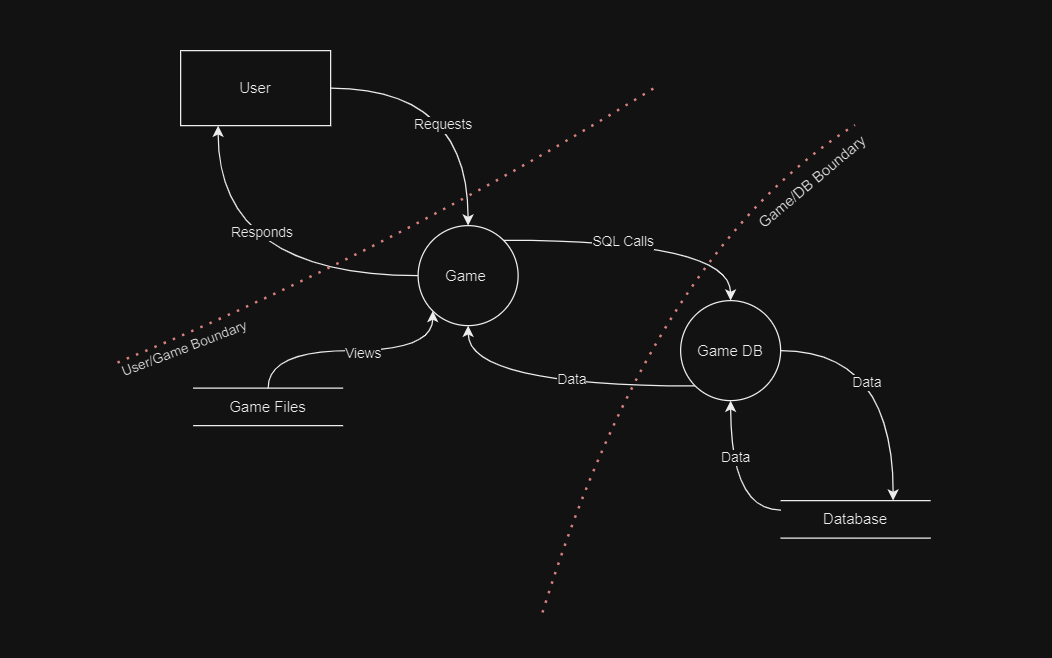
\includegraphics[width=1\textwidth]{diagrams/SecurityThreatModel.png}
    \caption{Model showing trust boundaries and security risks.}
    \label{security_threat_model}
\end{figure}

\subsubsection{Security Levels}
%250 words minimum
%Describe the different security levels for general users and administrators.  Also describe the authentication/authorization techniques for users of the software product.
For our game, there are only two types of users. We have the administrators, which are our team members, and the player, which are those who play the game. The administrators have the ability to access the backend of the game, so they can modify code, alter game design and so on. Another thing administrators can do is view the database where they can see all of the players’ login information and scores. Administrators have a separate login screen that is implemented in the Unity editor where they can log into the PlayFab account using the added PlayFab editor extension. Here we can also view data hidden from players. To see the overall user information, the administrator must access the account using the web browser. There you can see all of the player’s data as well as alter that data. They can also add and delete users and see logins, new users and API calls through the PlayFab account. 

The player only has the ability to see what the administrators allow the player to see. That goes for the login/registration pages, the start, the leaderboard and the actual gameplay view which includes the character. The player can only login using the in-game login system and can only view their personal information. The player can also view other players’ high scores on the leaderboard but are unable to edit that information. The player has the ability to play the game and upload scores to the database without accessing the database itself. 


%---------------------------End Product Security-------------------------------------------------

% No text here.

%---------------------------Product Performance-------------------------------------------------

\subsection{Product Performance}


\subsubsection{Product Performance Requirements}
%200 words minimum and list of performance non-functional requirements.
%Define and justify performance requirements.  These should be added to the list of non-functional requirements.
Many games have different attributes to make the performance as best as it could be. We decided that our game should run over 60 frames per second to make sure that no matter what happens, the game will be able to run as fast as it can. The CPU is at least 70\% at best. The operating system version for the player to play the game is Windows 7 and up for Windows, High Sierra 10.13+ for macOS, and Ubuntu 20.04 and 18.04 as well as CentOS 7 for Linux. The CPU needed for the game is 15 execution time but it sits at least 10 seconds in execution time. Analyzing and monitoring the software every few minutes also helps to ensure the game maintains high performance. For disk space, the player must have at least 80GB of space to make sure the game is functional.  The application is free for everyone to play on PC as well as Android and IOS. If needed, the user could also lower the resolution in the actual game to make things run smoother. The user must also make sure that the actual software can handle Unity games with a large disk space.  

\subsubsection{Measurable Performance Objectives}
%200 minimum words and list of objectives.
%Measurable Performance Objectives should be stated in this section that relate to the performance requirements.
The goal for this project was to recreate one level of the game Rampage. We decided to split the tasks up into parts like who will be responsible for sprites and controls of the main characters, NPCs and their scripts, login, etc. For this section of the project, we went with creating basic character scripts, adding sprites, and creating separate animations. With the many sprites that are present, we were self-aware of any that could take up disk space which could slow the work process on the game. To soften the blow of doing some tasks by ourselves, we also decided to look up YouTube videos to help give a guide on how to program the game. The main platform that the game is available on is the PC so to make things easier, the game is made with the control scheme of the keyboard. The next goal for the project was to go all into programming more complex parts of the code as well as doing more animations and making the NPCs functional. Sound was also be implemented at the same time as the other scripts were programed and there were ideas of having actual people doing the voices instead of just relying on sound effects. 

\subsubsection{Application Workload}
%250 words minimum
%Application Workload information should be gathered and visualized in this section.  This generally requires historical data on how the software product is being used.  For example, users generally spend 10% of the time interacting with menus, 80% of the time interacting with main features, 5% of the time saving work, etc.  These workloads should not be assumptions or guesses.  Timers need to be created for all major UI features of the product to generate reliable application workload analysis.
The user generally spends about 5\% of the game on the menu to at least start the game. About 75\% of the user’s time is spent in the actual game - destroying buildings and avoiding enemies. The login takes up at least up to another 5\%, it does not take long for the user to register an account which should take at least two minutes at best. As for system workload, the average time for the game to boot up is less than 10 seconds. The application for the game is mostly the one thing that is running on your computer for the best performance the user desires. Many applications not related to the game is more than likely cause bottlenecks in the background because they will cause either uneven CPU bottlenecks or GPU bottlenecks. They are running the software or on a hard drive if one possessed it. The loading time to get from one part of the game to another is also short and takea less than 10 seconds to load. The use of settings in the game depends on the user, but the user would likely spend another 5\% on settings. Our team hopes that the user has fun playing and plays with the best performance necessary. 

\subsubsection{Hardware and Software Bottlenecks}
%250 words minimum
%Hardware and Software Bottlenecks should be identified and discussed in this section, with test cases to justlify.
Bottlenecks vary depending on the computer and the space it uses. They mostly occur when either the CPU or the GPU holds back the potential of your software. Some of the issues that the user will likely encounter is high CPU when playing the game which could cause the game to slow down. To fix this problem, the users could do things like changing in-game settings by slowing down the graphics card to make sure that the rhythm matches the GPU, closing background programs by closing tasks in the task manager, overclocking RAM and CPU, etc. GPU bottlenecks can occur when the GPU card can calculate fewer images per second compared to the CPU. The way to fix a GPU bottleneck is by overclocking the component by increasing the temperature limit and increasing the clock speed, lowering the graphics in the game’s setting, or even by upgrading your GPU. You can also fix GPU bottlenecks by utilizing hardware monitoring tools as these can help you search for whatever is causing your system to slow down, as well as having a high-resolution monitor which demands equal power from both the CPU and GPU. If you are playing online, network bottlenecks can also occur. They happen when there are not enough resources to ensure reliable network data delivery. They can be fixed by upgrading your network by increasing your bandwidth and improving the architecture of the network. Another way to fix a network bottleneck is to divide your service plan by separating them into different sub-networks.


\subsubsection{Synthetic Performance Benchmarks}
%250 words minimum
%Synthetic Performance Benchmark test cases should be developed and executed on target hardware.  Results should be visualized and discussed in terms of the required target hardware details. (File I/O, CPU, Database).  Sysbench
The team used Sysbench to see results of how the game should run on our target platform, the PC. According to the first graph shown, the execution time for the CPU decreases around 32 threads. This is a good thing since it shows that execution of a program will be as quick as possible without it ruining the latency of the system. This will also benefit the actual game itself since the low execution time will make the game run smoothly without trouble. The throughput, in the second graph, measures how many units of information the system can process in each amount of time. If the throughput is low, the network will not be able to transfer large files and produce high rates of latency in the system. The read time is higher than the write time since it will take more time to read everything within certain files. The common pattern of both read and write time is that the throughput increases as the file size increases. The written time’s throughput increases from 3 to between 5 and 6 while read time’s throughput increases from between 4 and 5 to between 8 and 9. With the throughput being less than 10, it will ensure that loading certain assets of the game to the scene will be quick and sufficient for the user. It will also ensure that with the increase of the file size, the game will still run smoothly and will read files without ruining the CPU and GPU for the player and for the team.

%uncomment the section below when you're ready to insert an image
\begin{figure}[h!]
    \centering
    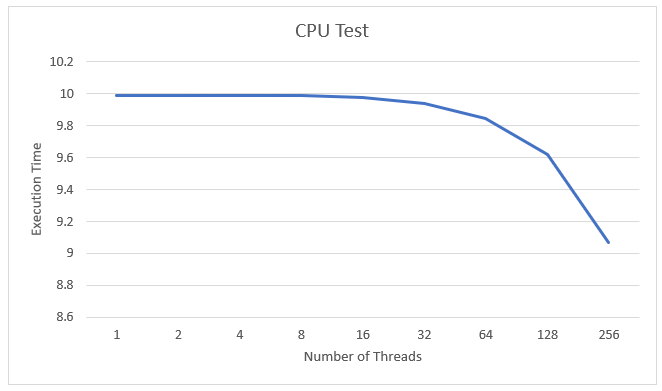
\includegraphics[width=1\textwidth]{diagrams/CPUTest.png}
    \caption{Graph depicting the number of threads vs execution time.}
    \label{cpu_test}
\end{figure}

%uncomment the section below when you're ready to insert an image
\begin{figure}[h!]
    \centering
    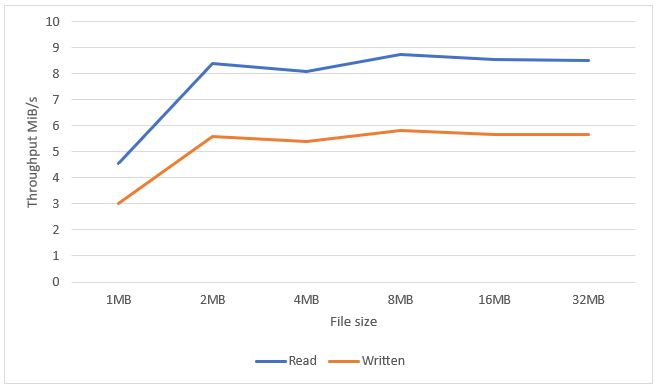
\includegraphics[width=1\textwidth]{diagrams/FileIOTest.png}
    \caption{Graph depicting file size vs throughput.}
    \label{fileio_test}
\end{figure}


\subsubsection{Performance Tests}
%250 words minimum and test case description with results
%Performance Test Cases should be given in this section.  Test Cases should be executed and results should be visualized (Images, Graphs, etc.)
%examples of performance tests include, but not limited to: Load testing (expected and peak loads, exceeding peak loads), Stress testing, throughput testing, function call timers, compatability testing, fault tolerance testing, etc.
Currently there are no visualization aid for most of these tests because they have yet to be implemented into the game. The tests are listed: \\

monsterRunTest: tests if the player can move left and right as well as jump 

monsterScaleBuilding: tests if the player can interact with the building by scaling it 

MonsterPunchTest: tests if the player can interact with the building by punching it

monsterDieAnimation: tests if the player has the right death animations 

building1ShowHoleTest: tests if building 1 can interact with the player by showing holes after the player punches them. 

building1CrumbleTest: tests if the buildings will execute the crumble animations once inflicted with enough holes 

building2ShowHoleTest: tests if building 1 can interact with the player by showing holes after the player punches them. 

building2CrumbleTest: tests if the buildings will execute the crumble animations once inflicted with enough holes 

building3ShowHoleTest: tests if building 1 can interact with the player by showing holes after the player punches them. 

building3CrumbleTest: tests if the buildings will execute the crumble animations once inflicted with enough holes 

soldierMoveTest: tests if the soldiers move a certain distance then move back to their spot.

soldierShootTest: tests if soldiers can shoot ammunition by command 

soldierDieTest: tests if the soldier dies when interacting with the player y being hit/squashed 

tankMoveTest: tests if the tanks move a certain distance then move back to their spot. 

tankShootTest: tests if tanks can shoot ammunition by command 

tankDieTest: tests if the tank dies when interacting with the player y being hit/squashed 

planeMoveTest: tests if the planes move a certain distance then move back to their spot. 

planeShootTest: tests if planes can shoot ammunition by command 

planeDieTest: tests if the plane dies when interacting with the player y being hit/squashed 

boomTest: tests if the boom sound effect works when properly called with some sort of damage inflicted by the player or the NPC 

crumbleTest: tests if the building crumbles when inflicted with a certain amount of damage 

RegisterTest: tests if the registration is successful 

loginTest: tests if the login is successful 

leaderboardDisplay: tests if the proper high score displays for the accounts registered in a leaderboard fashion 

highScoreChange: tests if the high score changes If new high score surpasses the old high score

healthCount: tests if the health depletes properly after damage is inflicted on the player 

healthDisplay: tests if the health depleting in the health bar is displayed 

pointCount: tests if the correct amount of points are added to the score


%---------------------------End Product Performance-------------------------------------------------

% No text here.


%---------------------------End Non-Functional Product Details Section---------------------------



% No text here.



%---------------------------Software Product Testing Section-------------------------------------
\section{Software Testing}



%---------------------------Software Testing Plan Template-------------------------------------

\subsection{Software Testing Plan Template}
%Each of the testing levels (unit, Integration, System, Acceptance) should use the following test plan template.

\textbf{Test Plan Identifier:} %Provides a unique identifier for the test. Every test should have a unique identification number for reference.

\textbf{Introduction:} % 50 words minimum. Brief description and objective about the test type.

\textbf{Test item:} %50 words minimum. Includes detailed information about the Software Under Test (SUT).

\textbf{Features to test/not to test:} %50 words minimum. In scope features. This could be newly added or updated features. Out of scope features not tested. [Provide reasoning for exclusion, like, non-impacted, low priority, etc.]

\textbf{Approach:} %50 words minimum. Strategy to test the software. Includes types of tests and how to test. Functional, performance, security testing using combined [manual + automation], manual only, automation only approach.

\textbf{Test deliverables:} %50 words minimum. All the deliverables from the testing e.g. approaches, test cases, reports etc.

\textbf{Item pass/fail criteria:} %50 words minimum. Entry and Exit criteria for all items. 

\textbf{Environmental needs:} %50 words minimum. Infrastructure required for SUT and executing test cases.

\textbf{Responsibilities:} %50 words minimum. Roles and responsibilities for various testing / supported activities.

\textbf{Staffing and training needs:} %50 words minimum. Training needs to bridge the gap of available and expected skill.

\textbf{Schedule:} %50 words minimum.  Test schedule should also be noted in the Gantt Chart. Test estimation (Efforts) and high-level schedule. Schedule should be for key deliverables or important milestones. Ideally, all test deliverables included in the test plan should be scheduled.

\textbf{Risks and Mitigation:} %100 words minimum. Risk identification for applicable items, assumptions, and mitigation plan.

\textbf{Approvals:} %Approvals and sign of dates.

%---------------------------Software Testing Plan Template-------------------------------------


% No text here.



%---------------------------Unit Testing-------------------------------------
\subsection{Unit Testing}
%copy of the completed Unit test plan should be placed here.
Text goes here.

\subsubsection{Source Code Coverage Tests}
%150 words minimum
%Insert Flow Graph Image(s).  Define cyclomatic complexity, basis paths, and Unit Test Cases
The  cyclomatic complexities of ChangeInput was 5. The cyclomatic complexities of HealthBarManager was 1. The cyclomatic complexities of PlayerMovements was 5. The cyclomatic complexities of PlayFabManager was 3. The cyclomatic complexities of ScoreManager was 1. The cyclomatic complexities of SoldierWalk was 3. See figures 27 through 32 in the appendix for images.

\begin{figure}[h!]
    \centering
    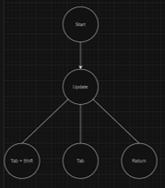
\includegraphics[width=1\textwidth]{diagrams/ChangeInputs.png}
    \caption{ChangeInputs complexity.}
    \label{inputs_chart}
\end{figure}

\begin{figure}[h!]
    \centering
    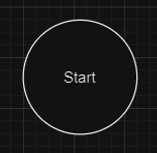
\includegraphics[width=1\textwidth]{diagrams/HealthBarManager.png}
    \caption{This table depicts the end results of our unit testing.}
    \label{unit_table}
\end{figure}

\begin{figure}[h!]
    \centering
    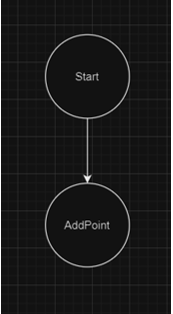
\includegraphics[width=1\textwidth]{diagrams/ScoreManager.png}
    \caption{ ads. }
    \label{score_manager}
\end{figure}

\begin{figure}[h!]
    \centering
    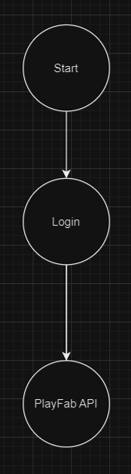
\includegraphics[width=1\textwidth]{diagrams/PlayFabManager.png}
    \caption{ sdf }
    \label{play_fab}
\end{figure}

\begin{figure}[h!]
    \centering
    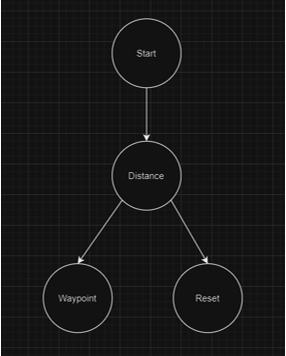
\includegraphics[width=1\textwidth]{diagrams/SoldierWalk.png}
    \caption{ sdf }
    \label{soldier_walk}
\end{figure}

\begin{figure}[h!]
    \centering
    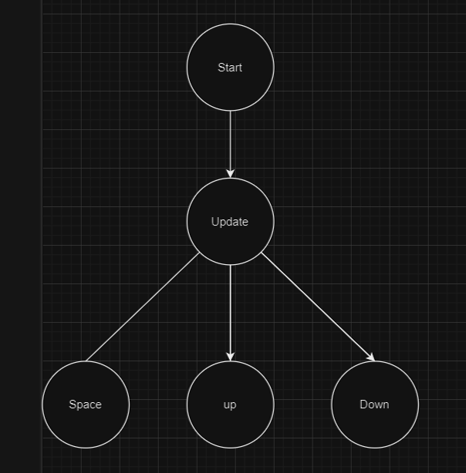
\includegraphics[width=1\textwidth]{diagrams/PlayerMovement.png}
    \caption{ sdf }
    \label{player_movement}
\end{figure}



\subsubsection{Unit Tests and Results}
%All unit tests results visualized (table, graph, etc.)
The table below depics the end results of our unit testing.
%uncomment the section below when you're ready to insert an image
\begin{figure}[h!]
    \centering
    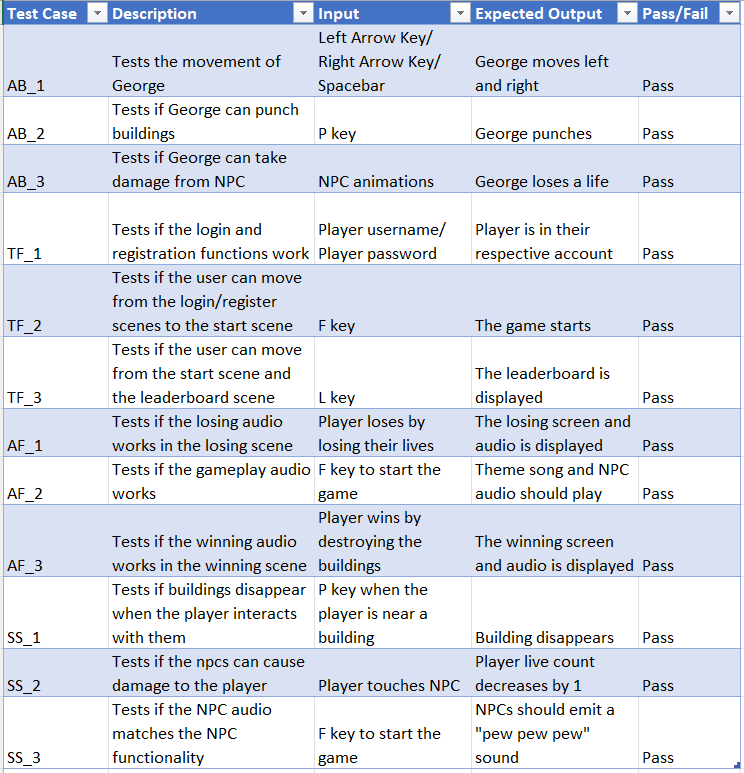
\includegraphics[width=1\textwidth]{diagrams/UnitTestingTable.png}
    \caption{This table depicts the end results of our unit testing.}
    \label{unit_table}
\end{figure}


%---------------------------End Unit Testing-------------------------------------

% No text here.

%---------------------------Integration Testing-------------------------------------
\subsection{Integration Testing}
%copy of the completed Integration test plan should be placed here.


\subsubsection{Integration Tests and Results}
%All integration tests results visualized (table, graph, etc.)
\textbf{Test Plan Identifier:} %Provides a unique identifier for the test. Every test should have a unique identification number for reference.
Integration Testing

\textbf{Introduction:} % 50 words minimum. Brief description and objective about the test type.
We used integration testing to combine the code and assets for our game. The main goal of using this is to combine every asset into one scene so we can fix any errors that surround the actual gameplay. The game should have a high and consistent framerate without changing settings.

\textbf{Test item:} %50 words minimum. Includes detailed information about the Software Under Test (SUT).
The main software we used to test data is on Unity, a game engine. The games created in Unity can be played on multiple platforms like PC, Switch, X-Box, etc. The planned system it will be tested on is PC and Mac since they are the easiest to grasp and understand. We also used Sysbench to view any drops in the CPU and GPU.

\textbf{Features to test/not to test:} %50 words minimum. In scope features. This could be newly added or updated features. Out of scope features not tested. [Provide reasoning for exclusion, like, non-impacted, low priority, etc.]
One of the main goals for the Rampage recreation is that the character should move left and right as well as jump and animations. We decided to exclude the environment as well as the environment size because they are low priority and the team wanted to focus on documentation and polishing the game more.

\textbf{Approach:} %50 words minimum. Strategy to test the software. Includes types of tests and how to test. Functional, performance, security testing using combined [manual + automation], manual only, automation only approach.
We tested the software by using the bottom-up method in which small parts of the program were tested before testing the main module. We had separate scenes to test the necessary parts before being put in the main scene. Then we would play it, find issues, and try to solve the code and its performance.

\textbf{Test deliverables:} %50 words minimum. All the deliverables from the testing e.g. approaches, test cases, reports etc.
We used Sysbench to detect any drops in framerates as well as to see if there were any bottlenecks that were present in the system. When inside the code, we would use debug log to make sure that every button-press and anything UI related would function correctly and will not hold back other aspects of the game.

\textbf{Item pass/fail criteria:} %50 words minimum. Entry and Exit criteria for all items. 
For entry criteria, before we start testing code, we must make sure that the test environment was set up and ready to code and the testable code was available. Exit criteria for this project is the deadline is met or most of the bug that were spotted in the code were fixed.

\textbf{Environmental needs:} %50 words minimum. Infrastructure required for SUT and executing test cases.
For the game to function, it must run on a Windows 10, Mac, or any up-to-date PC device. The system should also run on at least 64GB for optimal performance. It would be best to store the game on an external hard drive with at least 64GB or a regular computer with the same number of GB.

\textbf{Responsibilities:} %50 words minimum. Roles and responsibilities for various testing / supported activities.
One person was responsible for main menu, the other NPCS, and the other for the main character. Everyone on our team is responsible for testing their code and placement based on what they chose to work on. We are also responsible for giving each other feedback on any element that is not right when put into the main scene.

\textbf{Staffing and training needs:} %50 words minimum. Training needs to bridge the gap of available and expected skill.
The staff must have some coding experience, experience with C\#, or some familiarity with Unity. Anyone who doesn’t have any experience with C\# can get some insight from more experienced staff. The training will help with typing faster as well as being familiar with C\# to make progress faster. The staff must also be able to notice any bugs and report them to the developers or detect where the problem lies and edit them out.

\textbf{Schedule:} %50 words minimum.  Test schedule should also be noted in the Gantt Chart. Test estimation (Efforts) and high-level schedule. Schedule should be for key deliverables or important milestones. Ideally, all test deliverables included in the test plan should be scheduled.
Test schedule should also be noted in the Gantt Chart. Test estimation (Efforts) and high-level schedule. Schedule should be for key deliverables or important milestones. Ideally, all test deliverables included in the test plan should be scheduled. On November 21st to December 1st, we have been testing all codes for all assets. We would spend at least a few hours a day to make sure the player and menu are functioning as expected and that audio is present. At this moment, we are 50\% done with testing and we are now focusing on doing our documentation.

\textbf{Risks and Mitigation:} %100 words minimum. Risk identification for applicable items, assumptions, and mitigation plan.
When we implemented our assets into the same scene, we assumed that the game would cause a slow frame rate, and while some of that was true, the gravity of the characters would also mess up along with it. To fix these problems, we would have to turn off background apps and edit the gravity in the Unity menu. We also had to minimize any settings like graphics and controls which sped the game up significantly. For any errors in the code, we would look over and change certain aspects of it until the code, at least, somewhat works for what is intended of it.

\textbf{Approvals:} %Approvals and sign of dates.
As a team, we have all signed off and approved of all of our testing done on Nov. 29th with our client and Nov. 30th. 

\subsubsection{Integration Tests and Results}
%All integration tests results visualized (table, graph, etc.)
\begin{figure}[h!]
    \centering
    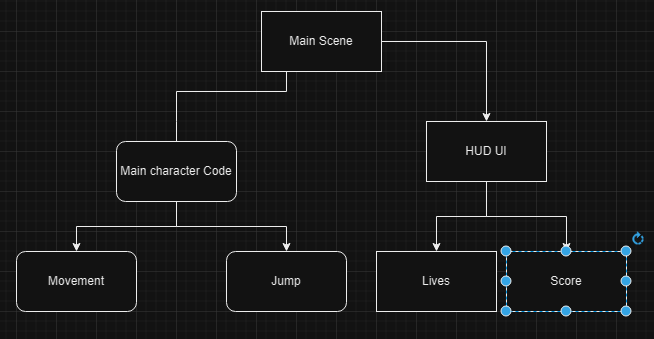
\includegraphics[width=1\textwidth]{diagrams/Integration_Visual.png}
    \caption{Integration testing visual.}
    \label{integration_testing}
\end{figure}



%---------------------------End Integration Testing-------------------------------------

% No text here.


%---------------------------System Testing-------------------------------------
\subsection{System Testing}
%copy of the completed System test plan should be placed here.

\textbf{Test Plan Identifier:} %Provides a unique identifier for the test. Every test should have a unique identification number for reference.
SystemTesting

\textbf{Introduction:} % 50 words minimum. Brief description and objective about the test type.
System testing is done to check the behaviour of the complete software based on software requirements. In this test, we will test whether the system functionalities are behaving as expected and specified in software requirements document, that the user interfaces are user friendly and easy to operate and use, and that the system guide is correct and complete.

\textbf{Test item:} %50 words minimum. Includes detailed information about the Software Under Test (SUT).
The software that we tested was a unity-made game that had numerous different functionalities, such as being able to login or register an account, viewing a leaderboard, and play the gameplay related to the game. The login/register and leaderboard scene use an external database to store and get its user data. We will test the functionality of these actions within the scene. 

\textbf{Features to test/not to test:} %50 words minimum. In scope features. This could be newly added or updated features. Out of scope features not tested. [Provide reasoning for exclusion, like, non-impacted, low priority, etc.]
The features that we tested were whether the user can register a new account or login with an existing account, do all of the scenes load as expected, and does the leaderboard get existing. We did not test whether there was a way for the user to cheat within the game and we did not check whether the game was compatible with other operating systems such as macOS because we ran out of time.  

\textbf{Approach:} %50 words minimum. Strategy to test the software. Includes types of tests and how to test. Functional, performance, security testing using combined [manual + automation], manual only, automation only approach.
For the functional testing, we played the game ourselves to ensure that it was functioning as expected. To test the login/register, we would register multiple accounts as well as login with those to ensure that multiple accounts are possible. For documentation testing, we would ensure that all of our documentation is accurate to what we implemented for the game. For usability testing, we would ensure that the game is user friendly.  

\textbf{Test deliverables:} %50 words minimum. All the deliverables from the testing e.g. approaches, test cases, reports etc.
Test cases for the system testing would be, “Is the user able to login/register an account?”, “Is the user able to switch from scenes?”, “Is the user able to play the game and win/lose?”, “Is the user able to see the leaderboard?” All of these tests passed and fulfilled the required function. 

\textbf{Item pass/fail criteria:} %50 words minimum. Entry and Exit criteria for all items. 
For the login/register scene to pass our needed criteria, the user would have to successfully register an account that will show up in online platform as well as be able to access that account when trying to login. For the loading of scenes, each scene would have to load successfully without errors. The leaderboard would also have to be able to access the database and obtain the leaderboard data. The player would also have to be able to win or lose within the actual gameplay. Otherwise, the tests would fail the criteria. 

\textbf{Environmental needs:} %50 words minimum. Infrastructure required for SUT and executing test cases.
For the software to run smoothly, the user would have to have access to Unity and a windows pc. We were unable to test whether it was playable on a Mac so we are unsure about that environment. The user would need to ensure that their system fulfilled all of the software requirements needed for Unity itself. 

\textbf{Responsibilities:} %50 words minimum. Roles and responsibilities for various testing / supported activities.
The documented software testing was done by Tameka. The team as a whole went through the various functions of the game to ensure they fulfilled what we had all expected. The database was entirely monitored and implemented by Tameka so testing involving the database was done and seen to by her. 

\textbf{Staffing and training needs:} %50 words minimum. Training needs to bridge the gap of available and expected skill.
The needed training would be learning more about system testing and how to go about the various types of system testing. Testing is an important part of software development so a better understanding on it would improve knowledge and skills significantly. To further increase software testing skills, we can utilise opportunities such as this course to help advance those skills.

\textbf{Schedule:} %50 words minimum.  Test schedule should also be noted in the Gantt Chart. Test estimation (Efforts) and high-level schedule. Schedule should be for key deliverables or important milestones. Ideally, all test deliverables included in the test plan should be scheduled.
For the software testing specifically, it was scheduled to be done by Nov. 30th. Based on the Gantt Chart, we scheduled and completed all of the prioritised tests during the last week of the sprint. This goes for the documentation for the testing as well as the test cases and their results. 

\textbf{Risks and Mitigation:} %100 words minimum. Risk identification for applicable items, assumptions, and mitigation plan.
A risk that could have transpired was that our database, if not implemented correctly, was not connected to our game. This would cause issues with logging in or registering as well as going further than the login/register scene. Additionally, if the database did not connect, there would be no way of viewing scores on the leaderboard either. To mitigate this, we would have to implement our database differently and not use an online platform to store user data. \\
Another risk would be that the system crashed due to errors within the code. This could be mitigated by code review and isolating where the issue is occurring. 

\textbf{Approvals:} %Approvals and sign of dates.
As a team, we have all signed off and approved of all of our testing done on Nov. 29th with our client and Nov. 30th. 


\subsubsection{System Tests and Results}
%All system tests results visualized (table, graph, etc.)

%uncomment the section below when you're ready to insert an image
\begin{figure}[h!]
    \centering
    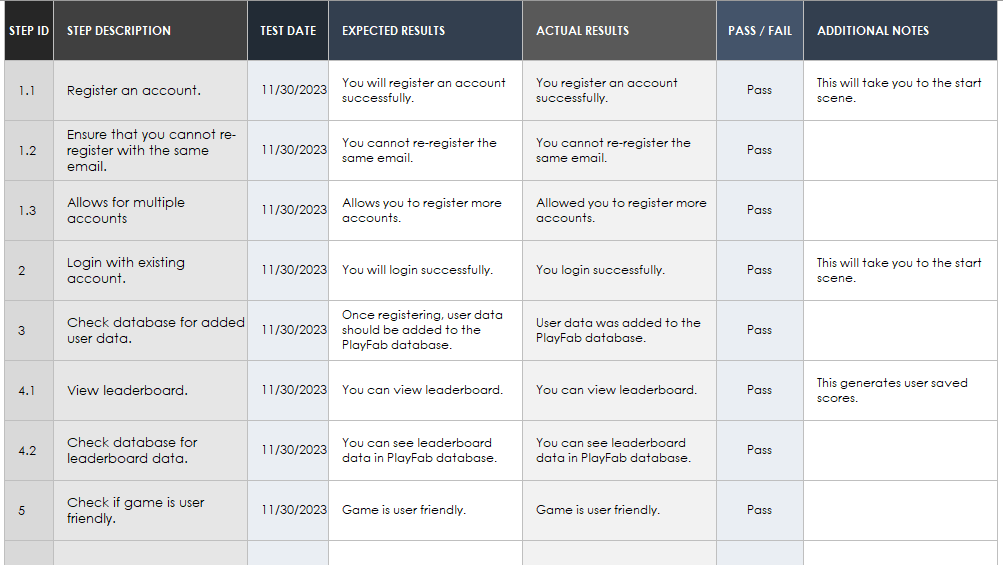
\includegraphics[width=1\textwidth]{diagrams/System_Testing_Results.png}
    \caption{System testing table results.}
    \label{system_testing}
\end{figure}


%---------------------------End System Testing-------------------------------------

% No text here.


%---------------------------Acceptance Testing-------------------------------------
\subsection{Acceptance Testing}
%copy of the completed Acceptance test plan should be placed here.
\textbf{Test Plan Identifier:} %Provides a unique identifier for the test. Every test should have a unique identification number for reference.
001-Acceptance

\textbf{Introduction:} % 50 words minimum. Brief description and objective about the test type.
The goal of the acceptance test is for our client to test the product and decide if it has been completed to their standards. The client was provided with a table of test cases and a column to mark as a pass, and a column to mark it as a fail. The objective is that the client is satisfied with the product and the development phase ends, moving forward into the maintenance of the product in the future.

\textbf{Test item:} %50 words minimum. Includes detailed information about the Software Under Test (SUT).
The test item is the software as a whole. Each scene is tested as a fully integrated system, with all audio, scripts, prefabs, etc. Each component of the system should be tested to ensure that the whole thing works properly and to the level the client desires. The start scene, login, register, playing scene, win, and lose scenes should all interact with each other as desired.

\textbf{Features to test/not to test:} %50 words minimum. In scope features. This could be newly added or updated features. Out of scope features not tested. [Provide reasoning for exclusion, like, non-impacted, low priority, etc.]
All features of the gameplay will be tested in the acceptance testing. Out of scope features are not tested but all features that are in the scope are tested. Character movement, scene changes, leaderboard functionality, login functionality, register functionality, and the win/lose conditions. That includes ensuring that the NPCs disappear when the player comes in contact with them and a life goes down. In turn, when the player touches the collision box on the buildings, the buildings disappear and the player gains a point.


\textbf{Approach:} %50 words minimum. Strategy to test the software. Includes types of tests and how to test. Functional, performance, security testing using combined [manual + automation], manual only, automation only approach.
The approach to the acceptance testing is to bring up the frst scene for the client and allow them to play through the game a few times to test different features. First, the client will test registering and logging into an account on the game. They will then test accessing the leaderboard and getting back to the main menu. Once back to the menu, they will play through the game and fulfill the winning conditions. After the win scene occurs, they will logout and try to register using the account they already created to see that it will not let them do that. They will then login with the account they made instead of registering it, and play the game again. This time they will fulfill the losing game conditions and see that the losing scene occurs. Throughout this, the client sees that the audio works, as well as each function we provided in the test case pass/fail table.


\textbf{Test deliverables:} %50 words minimum. All the deliverables from the testing e.g. approaches, test cases, reports etc.
The deliverable for this test is a table that contains three columns. The first column is the test case to be performed. The second column is to mark a check if the test case passed, aptly named "Pass". The last column, "Fail", is where the client will mark an X if the test was failed. The entire chart is completed at the final client/team meeting.


\textbf{Item pass/fail criteria:} %50 words minimum. Entry and Exit criteria for all items. 
Each test case involving moving from scene to scene requires that the client is able to move from one scene to another using the appropriate buttons/key presses wihtout issue in order to pass. If the client cannot do that then the test case failed. The testing of the player movement requires that the client is able to use AD or the left/right arrows keys to move George from side to side, and that the space bar makes George jump. If those actions occur as listed, the test is passed; otherwise it is a fail. For audio tests, if the audio plays without stopping, glitching, or beginning late then the test is passed. 



\textbf{Environmental needs:} %50 words minimum. Infrastructure required for SUT and executing test cases.
For the software to run smoothly, the user would have to have access to Unity and a windows pc. We were unable to test whether it was playable on a Mac so we are unsure about that environment. The user would need to ensure that their system fulfilled all of the software requirements needed for Unity itself. Beyond that, there are no other infrastructure requirements.


\textbf{Responsibilities:} %50 words minimum. Roles and responsibilities for various testing / supported activities.
It is the responsiblity of the team to bring a laptop containing the game/game environment to the client meeting for the client to test with. It also the responsibility of the team to bring a chart containing test cases and space to mark them as pass/fail for the client to use as they test. It is the responsibliity of the client to check the test cases against what is occuring as they move through the game and mark them as pass or fail; it is not the responsiblity of the team to check behind the client. 


\textbf{Staffing and training needs:} %50 words minimum. Training needs to bridge the gap of available and expected skill.
There is no staffing need for the acceptance testing. The training needs are those of understanding basic gameplay and gameplay mechanics. The client should have an understanding of game win and lose conditions, where to watch for those conditions to change, and how to navigate account creation, logins, and a leaderboard. 


\textbf{Schedule:} %50 words minimum.  Test schedule should also be noted in the Gantt Chart. Test estimation (Efforts) and high-level schedule. Schedule should be for key deliverables or important milestones. Ideally, all test deliverables included in the test plan should be scheduled.
The acceptance test will occur at the final client/team meeting of the semester. The meeting will take place on the twenty-eighth of November at three-thirty pm. The meeting is not expected to last any more than thirty minutes; at maximum the meeting could last to forty minutes until completetion of the acceptance testing.

\textbf{Risks and Mitigation:} %100 words minimum. Risk identification for applicable items, assumptions, and mitigation plan.
There are many risks within the acceptance testing. At any point a file could corrupt, which has the potential to derail the entire project. If a scene script corrupts that could entirely halt a section of gameplay and lead to multiple failed test cases, which would produce an overall failed product that does not meet the standards the client set forth. To avoid this, we have the project on a shared GitHub repository so that anyone can bring up the game on their laptop and switch it out if need be. Another risk that we face coming into the acceptance testing is that the internet is not working correctly. If the internet is not working, we cannot pull our project off of GitHub desktop to present to the client. Even if we could, our database could not function without the internet. If this does occur, we will use a phone from the group to start a hotspot and connect the laptop being used to that hotspot. This would allow us to pull the project off of GitHub and run it, as well as ensure that the database will be able to connect and function properly. 

\textbf{Approvals:} %Approvals and sign of dates.
The client, Dr. Galloway, approved of the acceptance test on November 28th. The team accepted the write-up on the acceptance test on December 1st.

\subsubsection{Acceptance Tests and Results}
%All Acceptance tests results visualized (table, graph, etc.)
%uncomment the section below when you're ready to insert an image
\begin{figure}[h!]
    \centering
    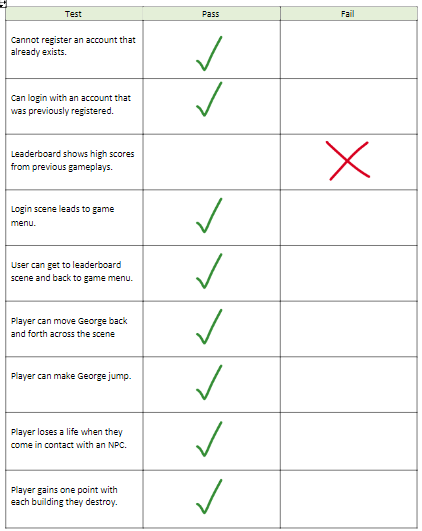
\includegraphics[width=1\textwidth]{diagrams/AcceptanceOne.png}
    \caption{Acceptance test table showing what test cases passed and failed.}
    \label{acceptance_test_table}
\end{figure}

\begin{figure}[h!]
    \centering
    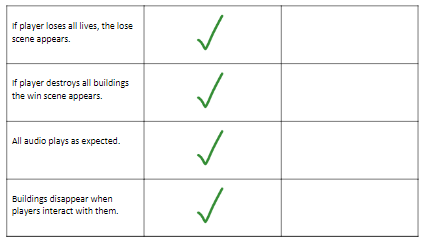
\includegraphics[width=1\textwidth]{diagrams/AcceptanceTwo.png}
    \caption{Acceptance test table showing what test cases passed and failed.}
    \label{acceptance_test_tabletwo}
\end{figure}

%---------------------------End System Testing-------------------------------------

% No text here.





%---------------------------End Software Product Testing Section-------------------------------------


% No text here.



%---------------------------Conclusion Section-------------------------------------
\section{Conclusion}
%300 words minimum
%Concluding remarks that summarizes the purpose and outcomes of the technical document.  Discussion of short comings and future work.
The purpose of the technical document for this project, Rampage, is to ensure a complete understanding of how the project has been designed and created. This ensures that should anyone new come onto the project they could be completely up to date by reading this documention, as well as ensuring that should the project ever need to be replicated again that it can be. This document includes all of the design patterns, creation information, source code, etc., that would be needed to completely replicate this project. Truthfully, the real outcome of creating this documentation thus far has been a deeper understanding across the team of what this project is meant to accomplish – the scope, the functionality requirements, etc. It has also been a great way to check that we are building the product the way that we should be. While creating this documentation, we would check our designs and plans for implementation against what the client was expecting. That really enabled us to keep ourselves on that designated track. In terms of the team’s shortcomings, there were a few that cropped up in sprints three and four. We found that not everyone on the team had a strong grasp on how to navigate and use the Unity game engine for development, which caused issues at every point along the way. We also found that not everyone was familiar with C Sharp; we hadn’t planned on that and thus had not allocated ourselves enough time to learn it as thoroughly as needed. The last shortcoming that seemed to have a stronger impact on both the team and this project was a lack of necessary and thorough communication.  Without clear and proper communication, portions of the project were harder to integrate together, and the expectations of each member were not always clear. If we were to continue this work in the future, we would need to target these issues before continuing on to ensure that they would not stand in the way of creating the best product as possible for our client. 

%---------------------------End Conclusion Section-------------------------------------


% No text here.



%---------------------------Appendix Section-------------------------------------------
\section{Appendix}

\subsection{Software Product Build Instructions}
%Include in this section all steps for copying the current state of the product to new computers for continued development.
To build our project, ensure that you have Unity installed. We are using the 2022.3.11f1 editor version so ensure that that editor us also installed on Unity. To find our shared project file, you can find it on GitHub under MikaMika2003/Rampage. From there download the zip file and open it in your unity hub. Once that opens, you should have the current state of our software product. 

\subsection{Software Product User Guide}
%Include in this section an overview guide on how to use your software product for a general user and an administrative user.
As an admin user, you can log into the PlayFab database using the shared username and password to view the database. Go to PlayFab.com. Here you can view the players that have registered and the leaderboard for scores. As admin, you can also delete remove users and change user information. 
As a user, you can launch the game where you can either register or login to an account. After, you will be met with the start menu and you can press 'F' to start the game or 'L' to view leaderboard. Once the game is started you have to either destroy all buildings or come in contact with the npcs to be met with the game over scene. From there you can logout and login again if you wish to restart the game. 

\subsection{Source Code with Comments}
%Include in this section all final source code for the product.  Label each file with headings such as, C.1 file1.c, C.2 file2.c, C.3 file1.py, etc.  All source code should be effectively commented.

\subsubsection{ChangeInputs.cs}

\begin{verbatim}
using System.Collections;
using System.Collections.Generic;
using UnityEngine;
using UnityEngine.UI;
using UnityEngine.EventSystems;

public class ChangeInputs : MonoBehaviour
{

    EventSystem system1;
    public Selectable firstInput;
    public Button submitBtn; 

    // Start is called before the first frame update
    void Start()
    {
        system1 = EventSystem.current;
        firstInput.Select();
    }

    // Update is called once per frame
    // This is for when the user clicks tab to go to the next input field
    void Update()
    {
        // Checks if the tab and left shift is clicked
        if (Input.GetKeyDown(KeyCode.Tab) && Input.GetKey(KeyCode.LeftShift)) {
            Selectable previous = system1.currentSelectedGameObject.GetComponent<Selectable>().FindSelectableOnUp();
            if(previous != null) {
                previous.Select();
            }
        }
        // Checks if the tab is clicked
        else if (Input.GetKeyDown(KeyCode.Tab)) {
            Selectable next = system1.currentSelectedGameObject.GetComponent<Selectable>().FindSelectableOnDown();
            if(next != null) {
                next.Select();
            }
        }
        // Checks if the enter button is clicked 
        else if (Input.GetKeyDown(KeyCode.Return)) {
            submitBtn.onClick.Invoke();
            Debug.Log("Button pressed!");
        }
    }
}
\end{verbatim}


\subsubsection{PlayFabManager.cs}

\begin{verbatim}
using System.Collections;
using System.Collections.Generic;
using UnityEngine;
using PlayFab.ClientModels;
using PlayFab;
using System;
using UnityEngine.UI;
using Unity.VisualScripting;
using UnityEngine.SceneManagement;

// This class is used for interacting with our PlayFab database
public class PlayFabManager : MonoBehaviour
{
    [Header("UI")]
    public Text messageText;
    public InputField emailInput;
    public InputField passwordInput;
    public Button registerBtn;
    public Button loginBtn;
    public Button Get_LB_Btn; 
    public Button Back_Btn;


    void Start()
    {
        // Assign the RegisterButton method to the button's onClick event
        if (registerBtn != null)
        {
            registerBtn.onClick.AddListener(RegisterButton);
        }

        if (loginBtn != null)
        {
            loginBtn.onClick.AddListener(LoginButton);
        }
        if (Get_LB_Btn != null) 
        {
            Get_LB_Btn.onClick.AddListener(GetLeaderboard);
        }
        if (Back_Btn != null) 
        {
            Back_Btn.onClick.AddListener(BackToStartScene);
        }

        AddRandomDataToLeaderboard();
        
        

    }

    // Scene manager that takes the user back to the start scene
    public void BackToStartScene() {
        SceneManager.LoadScene("StartScene");
    }

    // If the register and login button is pressed, it checks to ensure that the inputs are valid
    public void RegisterButton() {

        if (passwordInput.text.Length < 6) {
            messageText.text = "Password too short!";
            return;
        }

        var request = new RegisterPlayFabUserRequest {
            Email = emailInput.text, 
            Password = passwordInput.text,
            RequireBothUsernameAndEmail = false 
        };
        PlayFabClientAPI.RegisterPlayFabUser(request, OnRegisterSuccess, OnRegisterError);
    }

    void OnRegisterSuccess(RegisterPlayFabUserResult result)
    {
        messageText.text = "Registered and logged in!";
        Debug.Log("PlayFab User ID: " + result.PlayFabId);
        SceneManager.LoadScene("StartScene");
    }

    void OnRegisterError(PlayFabError error)
    {
        messageText.text = error.ErrorMessage;
        Debug.Log(error.GenerateErrorReport());
    }


    // If the login button is pressed then it checks user validation within the PlayFab database
    public void LoginButton() {
        var request = new LoginWithEmailAddressRequest {
            Email = emailInput.text, 
            Password = passwordInput.text
        };
        PlayFabClientAPI.LoginWithEmailAddress(request, OnLoginSuccess, OnLoginError);
    
    }

    void OnLoginSuccess(LoginResult result)
    {
        messageText.text = "Logged in!";
        Debug.Log("Successful login/create account!");
        SceneManager.LoadScene("StartScene");
    }

    void OnLoginError(PlayFabError error)
    {
        messageText.text = error.ErrorMessage;
        //Debug.Log("Error while logging in/creating account!");
        Debug.Log(error.GenerateErrorReport());
    }


    // 
    void OnError(PlayFabError error)
    {
        //messageText.text = error.ErrorMessage;
        Debug.Log("Error while getting leaderboard");
        Debug.Log(error.GenerateErrorReport());
    }

    public GameObject rowPrefab;
    public Transform rowsParent;
    
    // Method to add random data to the leaderboard
    public void AddRandomDataToLeaderboard()
    {
        int numberOfEntries = 5; // Adjust this based on the number of entries you want to add

        for (int i = 0; i < numberOfEntries; i++)
        {
            // Generate a random score
            int randomScore = UnityEngine.Random.Range(0, 3);

            // Call the method to send the random score to the leaderboard
            SendLeaderboard(randomScore);
        }

        // After adding the random data, refresh the leaderboard

        GetLeaderboard();
    }

    
    // For leaderboard scores to send to PlayFab
    public void SendLeaderboard(int score) {
        var request = new UpdatePlayerStatisticsRequest {
            Statistics = new List<StatisticUpdate> {
                new StatisticUpdate {
                    StatisticName = "GainedPoints",
                    Value = score
                }
            }
        };
        PlayFabClientAPI.UpdatePlayerStatistics(request, OnLeaderboardUpdate, OnError);
    }

    // If the score is updated it updates the leaderboard
    void OnLeaderboardUpdate(UpdatePlayerStatisticsResult result)
    {
        Debug.Log("Successful leaderboard sent!");       

        // Check if the "B" key is pressed
        if (Input.GetKeyDown(KeyCode.B))
        {
            // Load your target scene
            SceneManager.LoadScene("StartScene");
        }
    }
 

    // Gets the leaderboard
    public void GetLeaderboard() {
        Debug.Log("Attempting to get leaderboard...");
        Get_LB_Btn.interactable = false;


        var request = new GetLeaderboardRequest {
            StatisticName = "GainedPoints",
            StartPosition = 0,
            MaxResultsCount = 10
        };
        PlayFabClientAPI.GetLeaderboard(request, OnLeaderboardGet, OnError);
    }

    // Shows the leaderboard
    // Gets all the information like position, player name and score for each entry
    void OnLeaderboardGet(GetLeaderboardResult result)
    {

        Get_LB_Btn.interactable = true;

        // Remove all existing rows
        foreach (Transform item in rowsParent) {
            Destroy(item.gameObject);
        }

        foreach (var item in result.Leaderboard) {
            GameObject newGo = Instantiate(rowPrefab, rowsParent);
            Text[] texts = newGo.GetComponentsInChildren<Text>();

            // Get position on leaderboard, then player id then player score
            texts[0].text = (item.Position + 1).ToString();
            texts[1].text = item.PlayFabId;
            texts[2].text = item.StatValue.ToString();

            Debug.Log(string.Format("PLACE: {0} | ID: {1} | VALUE: {2} ", 
            item.Position + 1, item.PlayFabId, item.StatValue));
        }
    }   
}
\end{verbatim}


\subsubsection{OpenGame.cs}

\begin{verbatim}
using System.Collections;
using System.Collections.Generic;
using UnityEngine;
using UnityEngine.SceneManagement;
using TMPro;

public class OpenGame : MonoBehaviour
{
    // Update is called once per frame
    void Update()
    {
        // Check if the "F" key is pressed
        if (Input.GetKeyDown(KeyCode.F))
        {
            // Load your target scene
            SceneManager.LoadScene("PlayingScene");
        }

        // Check if the "L" key is pressed
        if (Input.GetKeyDown(KeyCode.L))
        {
            // Load your target scene
            SceneManager.LoadScene("Leaderboard");
        }
    }
}
\end{verbatim}

\subsubsection{PlayerMovement.cs}

\begin{verbatim}
using System.Collections;
using System.Collections.Generic;
using UnityEngine;

// This file is used to control the main character's movements
public class PlayerMovement : MonoBehaviour
{
    private float horizontal;
    public float speed = 15f;
    public float jumpForce = 30f;
    private bool isFacingLeft = true;

    [SerializeField] private Rigidbody2D rb;
    [SerializeField] private Transform groundCheck;
    [SerializeField] private LayerMask groundLayer;  
    [SerializeField] private Animator animator;


    // On start it gets the character and places it within the scene
    void Start()
    {
        rb = GetComponent<Rigidbody2D>();
    }
    
    // This used to determine and update the current  movement of the player 
    void Update()
    {
        horizontal = Input.GetAxisRaw("Horizontal");
        Flip();
        animator.SetFloat("Speed", Mathf.Abs(horizontal));

        // Checks if the up key is pressed 
        if(Input.GetKey("up"))
        {
            animator.SetBool("LookingUp", true);
        } else
        {
            animator.SetBool("LookingUp", false);
        }

        // Checks if the down key is pressed
        if(Input.GetKey("down"))
        {
            animator.SetBool("LookingDown", true);
        } else
        {
            animator.SetBool("LookingDown", false);
        }

        // Checks if the z key is pressed
        if(Input.GetKeyDown(KeyCode.Z))
        {
            animator.SetBool("IsPunching", true);
            StartCoroutine(WaitSecond());
            animator.SetBool("IsPunching", false);
        }

        rb.velocity = new Vector2(horizontal * speed, rb.velocity.y);

        Jumping();
    }

    // Introduces a wait period for character movement
    IEnumerator WaitSecond(){
        yield return new WaitForSeconds(1);
    }

    // Checks if the space button is pressed 
    private void Jumping()
    {
        animator.SetBool("IsJumping", !isGrounded()); 

        if(Input.GetButtonDown("Jump") && isGrounded())
        {
            rb.velocity= new Vector2(rb.velocity.x, jumpForce);
            
        }
    }


    // Keeps the character grounded to the added platform 
    private bool isGrounded()
    {
        return Physics2D.OverlapCircle(groundCheck.position, 0.2f, groundLayer);
    } 

    // Checks the direction in which the character is facing
    private void Flip()
    {
        if (isFacingLeft && horizontal > 0f || !isFacingLeft && horizontal < 0f)
            {
                isFacingLeft = !isFacingLeft;
                Vector3 localScale = transform.localScale;
                localScale.x *= -1f;
                transform.localScale = localScale;
            
        }

    }
}
\end{verbatim}

\subsubsection{HealthBarManager.cs}

\begin{verbatim}
using System.Collections;
using System.Collections.Generic;
using UnityEngine;
using UnityEngine.UI;

// This class was not used

public class HealthBarManager : MonoBehaviour
{
    
    // slider for the health bar 
    Slider _healthSlider;

    // Gets the slider component
    private void Start()
    {
        _healthSlider = GetComponent<Slider>();
    }

    // sets the max health possible
    public void SetMaxHealth(int maxHealth)
    {
        _healthSlider.maxValue = maxHealth;
        _healthSlider.value = maxHealth;
    }

    // sets the health value 
    public void SetHealth(int health)
    {
        _healthSlider.value = health;
    }


}
\end{verbatim}

\subsubsection{ScoreManager.cs}

\begin{verbatim}
using System.Collections;
using System.Collections.Generic;
using UnityEngine;
using UnityEngine.UI;

public class ScoreManager : MonoBehaviour
{
    public static ScoreManager instance;

    public Text scoreText;

    int score = 0;

    // Call the database to get the highscore and set it to highscore
    // int highscore = 0;


    // This will be called at the very start of the game before Start() is called
    // Will set an instance of the Manager that can be used in other classes
    private void Awake()
    {
        instance = this;
    }

    // Start is called before the first frame update
    void Start()
    {
        scoreText.text = score.ToString();
    }


    public void AddPoint()
    {
        //score += 1 //or however many points should be added
        scoreText.text = score.ToString();

        // To save the highscore
        //if (hignscore < score) 
        //    PlayerPrefs.SetInt("hignscore", score);
      
    }
}
\end{verbatim}


%---------------------------End Appendix Section-------------------------------------------














%example image:  uncomment to show usage
%\begin{figure}[h]
%    \centering
%    \includegraphics[width=1\textwidth]{images/Add_non-music.png}
%    \caption{This is how you add non-music items.}
%    \label{fig16}
%\end{figure}


%example links:  uncomment to show usage.
%\url{https://www.youtube.com}
%\href{https://www.wku.edu/}{WKU Homepage}
%\footnote{You can put the link in a footnote like this.}

% Anything to the right of a percent sign will be ignored by LaTeX.
% You can use this to put notes to yourself.  



\end{document}
